\documentclass[graybox]{svmult}

\usepackage[utf8]{inputenc}
\usepackage[small,bf]{caption}
\usepackage{amssymb}
\usepackage{amstext}
\usepackage{mathtools}
\usepackage{mathptmx}       
\usepackage{helvet}        
\usepackage{courier}      
\usepackage{type1cm}     
\usepackage{listings}                        
\usepackage{makeidx}    
\usepackage{graphicx}   
\usepackage{multicol}        
\usepackage[bottom]{footmisc}
\usepackage[spanish]{babel}
\usepackage[T1]{fontenc} 

% For the way captions are centered
\setlength{\captionmargin}{27pt}

\overfullrule=1mm

%%% for Spanish
\def\abstractname{Resumen}%
\def\ackname{Agradecimientos}%
\def\andname{y}%
\def\bibname{Referencias}%
\def\lastandname{, y}%
\def\appendixname{Apéndice}%
\def\chaptername{Capítulo}%
\def\claimname{Afirmación}%
\def\conjecturename{Conjetura}%
\def\contentsname{Contenidos}%
\def\corollaryname{Corolario}%
\def\definitionname{Definici\'on}%
\def\emailname{e-mail}%
\def\examplename{Ejemplo}%
\def\examplesname{Ejemplos}%
\def\exercisename{Ejercicio}%
\def\figurename{Fig.}%
\def\forewordname{Foreword}%
\def\keywordname{{\bf Palabras clave:}}%
\def\indexname{Índice}%
\def\lemmaname{Lema}%
\def\listfigurename{Figuras}%
\def\listtablename{Tablas}%
\def\notename{Nota}%
\def\partname{Parte}%
\def\prefacename{Prefacio}%
\def\problemname{Problema}%
\def\proofname{Demostración}%
\def\propertyname{Propiedad}%
\def\propositionname{Proposici\'on}%
\def\questionname{Pregunta}%
\def\refname{Referencias}%
\def\remarkname{Observación}%
\def\seename{see}%
\def\solutionname{Solución}%
\def\tablename{Tabla}%
\def\theoremname{Teorema}
\def\notationname{Notación}
\def\conventionname{Convención}

% % change numbers 
\let\remark\relax
\let\theorem\relax
\let\lemma\relax
\let\definition\relax
\let\proposition\relax
\let\corollary\relax
\let\exercise\relax
\let\example\relax
\let\conjecture\relax
\spnewtheorem{theorem}{\theoremname}{\bfseries}{\itshape}
\renewcommand\thetheorem{\arabic{theorem}}
\spnewtheorem{lemma}[theorem]{\lemmaname}{\bfseries}{\itshape}
\spnewtheorem{definition}[theorem]{\definitionname}{\bfseries}{\itshape}
\spnewtheorem{proposition}[theorem]{\propositionname}{\bfseries}{\itshape}
\spnewtheorem{corollary}[theorem]{\corollaryname}{\bfseries}{\itshape}
\spnewtheorem{exercise}[theorem]{\exercisename}{\bfseries}{\upshape}
\spnewtheorem{example}[theorem]{\examplename}{\bfseries}{\upshape}
\spnewtheorem{examples}[theorem]{\examplesname}{\bfseries}{\upshape}
\spnewtheorem{remark}[theorem]{\remarkname}{}{\upshape}
\spnewtheorem{conjecture}[theorem]{\conjecturename}{\bfseries}{\upshape}
\spnewtheorem{notation}[theorem]{\notationname}{\bfseries}{\upshape}
\spnewtheorem{convention}[theorem]{\conventionname}{\bfseries}{\upshape}

\newcommand{\N}{\mathbb{N}}
\newcommand{\B}{\mathbb{B}}
\newcommand{\Q}{\mathbb{Q}}
\newcommand{\Z}{\mathbb{Z}}
\newcommand{\F}{\mathbb{F}}
\newcommand{\R}{\mathbb{R}}
\newcommand{\C}{\mathbb{C}}
\newcommand{\K}{\mathbb{K}}
\newcommand{\T}{\mathbb{T}}

\newcommand{\FK}{\mathcal{E}}
\newcommand{\NA}{\mathfrak{B}}
\newcommand{\ad}{\mathrm{ad}}
\newcommand{\charK}{\mathrm{char}{\K}}
\newcommand{\supp}{\mathrm{supp}}
\newcommand{\ydG}{\prescript{G}{G}{\mathcal{YD}}}
\newcommand{\ydH}{\prescript{H}{H}{\mathcal{YD}}}

%%% Definitions
\newcommand{\Aff}{\mathrm{Aff}}
\newcommand{\Rad}{\mathrm{rad}}
\newcommand{\Inn}{\mathrm{Inn}}
\newcommand{\Stab}{\mathrm{Stab}}
\newcommand{\Ext}{\mathrm{Ext}}
\newcommand{\Img}{\mathrm{Img}}
\newcommand{\Conj}{\mathrm{Conj}}
\newcommand{\fix}{\operatorname{fix}}
\newcommand{\soc}{\operatorname{soc}}
\newcommand{\id}{\operatorname{id}}
\newcommand{\op}{\operatorname{op}}
\newcommand{\cop}{\operatorname{cop}}
\newcommand{\rk}{\operatorname{rk}}
\newcommand{\Aut}{\operatorname{Aut}}
\newcommand{\End}{\operatorname{End}}
\newcommand{\Irr}{\operatorname{Irr}}
\newcommand{\img}{\operatorname{img}}
\newcommand{\GL}{\mathbf{GL}}
\newcommand{\SL}{\mathbf{SL}}
\newcommand{\PGL}{\mathrm{PGL}}
\newcommand{\PSL}{\mathrm{PSL}}
\newcommand{\PSU}{\mathrm{PSU}}
\newcommand{\Sz}{\mathrm{Sz}}
\newcommand{\Ree}{\mathrm{Ree}}
\newcommand{\Sp}{\mathrm{Sp}}
\newcommand{\Alt}{\mathbb{A}}
\newcommand{\Sym}{\mathbb{S}}
\newcommand{\ord}{\mathrm{ord}}


\makeindex             
                      
\begin{document}

\lstset{language=GAP,
  showstringspaces=false,
  xleftmargin=0.0cm,
  xrightmargin=0.0cm,
  basicstyle=\small\ttfamily,
  frame=single,
  framerule=0pt,
}

\title*{Nudos, quandles y homología}
\author{Leandro Vendramin}

\institute{Leandro Vendramin \at Vrije Universiteit Brussel, \email{Leandro.Vendramin@vub.be}}

\maketitle

\abstract{
Presentamos una introducción informal a la teoría combinatoria de nudos.
Discutiremos el grupo fundamental de un nudo, invariantes por coloreo e
invariantes dados por quandles y homología de quandles.
}

\section{Introducción}

Robert Graves\footnote{R. Graves, Los mitos griegos, Alianza Editorial, 1996.}
cuenta una leyenda griega en la que un oráculo anunció a los habitantes de
Frigia que reconocerían a su futuro rey al verlo llegar en una carreta de
bueyes.  Tiempo después, el pueblo reconoció en un campesino de nombre Gordias
a su nuevo rey. En agradecimiento, Gordias ofreció a Zeus su carro y el yugo,
que había atado con un nudo tan complicado que nadie podría desatar. Se dijo
que el que fuera capaz de desatar el nudo de Gordias conquistaría Asia.  Siglos
después, Alejandro Magno tuvo que enfrentarse al reto de desatar ese nudo y,
sin vacilación, deshizo el nudo al cortar la cuerda con su espada.  Según se
dice, esa misma noche, Zeus, con una fuerte tormenta, mostró su aprobación a la
solución encontrada por Alejandro Magno.

\begin{figure}
    \centering
	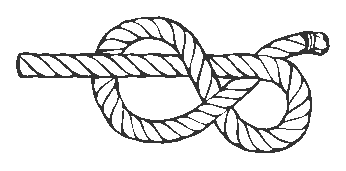
\includegraphics[scale=0.6]{images/rope}
\end{figure}

La teoría de nudos, en principio, intenta entender los nudos que podríamos
encontrarnos en la vida real. 
El objetivo final de la teoría es obtener una clasificación completa de los nudos, salvo
deformaciones continuas. A simple vista, uno podría pensar entonces
que la teoría de nudos es una divertida rama de la topología. Si bien esto es
cierto, es necesario destacar que el estudio de los nudos se lleva a
cabo gracias al uso de técnicas muy profundas que provienen de distintas ramas
de la matemática como la geometría, el álgebra y el análisis. La teoría de
nudos tiene además muchas aplicaciones en otras ciencias, entre ellas la biología, la
física y la criptografía. 

Invitamos al lector a que tome un pedazo de cuerda y haga un nudo tal como el
que vemos a la izquierda en la figura~\ref{fig:nudo}. Si pegamos los extremos
de esa cuerda obtendremos una cuerda anudada que no tiene extremos tal como la
que vemos a la derecha en misma figura.

\begin{figure}
    \centering
	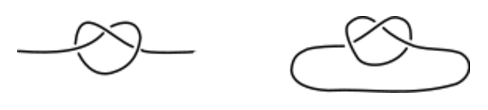
\includegraphics[scale=0.7]{images/real}
    \caption{Nudos.}
    \label{fig:nudo}
\end{figure}

\textquestiondown Puede desatarse ese nudo? Después de varios minutos de
experimentación se hace más o menos evidente que ese nudo podrá deshacerse
solamente si nos permitimos cortar la cuerda. Sin embargo, si aceptamos
soluciones como la que encontró Alejandro Magno, entonces todo nudo puede
desatarse y el problema de clasificar nudos --que bajo estas condiciones resulta ser muy poco
interesante-- queda resuelto: todo nudo es trivial.  

\textquestiondown Qué pasa si no está permitido cortar cuerdas?
\textquestiondown Cómo podríamos demostrar matemáticamente que un nudo no puede
desatarse?  Para responder esta pregunta, primero es necesario describir
matemáticamente un nudo de forma tal que la definición permita modelar con
cierta fidelidad el fenómeno real de anudar una cuerda. Necesitamos además que
nuestra definición excluya patologías matemáticas desagradables tales como
hacer desaparecer un nudo al tirar indefinidamente de los extremos de la
cuerda.  Por último, necesitamos una definición precisa y acertada de lo que
significa que dos nudos sean \emph{equivalentes}, es decir iguales aunque se
vean distintos. Una vez que tengamos estas cosas, habremos formulado
matemáticamente el problema de estudiar nudos, y entonces, tal como se hace en
muchas ramas de la matemática, podremos concentrarnos en estudiar nudos
mediante el uso de invariantes. 

\subsection*{Agradecimientos}

Este texto corresponde a un minicurso dictado en el Encuentro Nacional de
Álgebra, elENA VII, La Falda, Córdoba, Argentina, 2014.  Agradezco a Agustín
García, Jonathan Barmak, Edwin Clark, Marco Farinati, César Galindo, Juliana
García Galofre, César Massri y Masahico Saito los comentarios y las
correcciones. Para terminar, quiero expresar mi agradecimiento a un anónimo y
cuidadoso revisor; sus comentarios fueron de gran ayuda. 

\section{Nudos}
\label{section:knots}

Esta primera sección está dedicada a los conceptos básicos de la teoría de
nudos y al teorema de Reidemeister, que nos permite traducir el problema
topológico de distinguir nudos al lenguaje de la combinatoria. 

\begin{figure}[h]
	\centering
    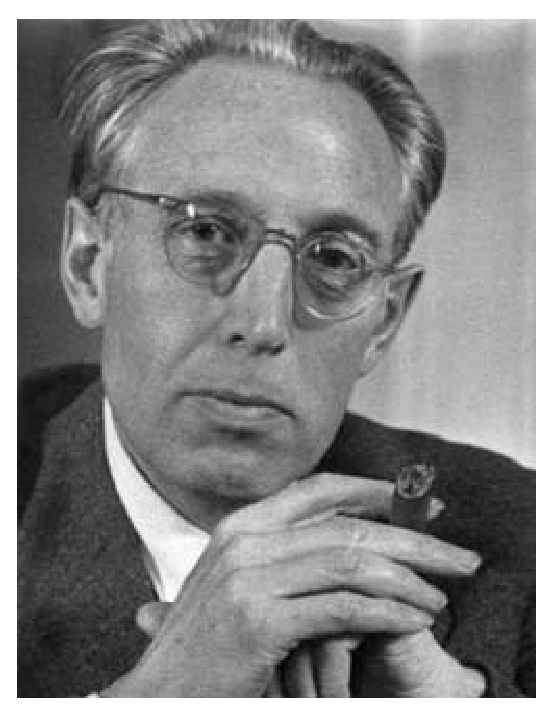
\includegraphics[width=30mm,height=36mm]{images/reidemeister}
    \caption{Kurt Reidemeister (1893--1971)}
\end{figure}

\begin{definition}
    \index{Nudo}
    Un \textbf{nudo} (en $\R^3$) es 
	una función inyectiva y continua $S^1\to\R^3$, donde
	$S^1=\{(x,y)\in\R^2\mid x^2+y^2=1\}$ es la circunferencia. 
\end{definition}

En el conjunto de nudos definimos la relación de equivalencia dada por
\textbf{isotopía}. 

\begin{definition}
	\index{Equivalencia de nudos}
	Diremos que los nudos dados por las funciones $\alpha$ y $\beta$ son
	\textbf{equivalentes} si y sólo si existe una función continua $H\colon
	S^1\times[0,1]\to\R^3$ tal que la función $H_t\colon z\mapsto H(z,t)$ es un
	nudo para todo $t\in [0,1]$, $H_0=\alpha$ y $H_1=\beta$. 
\end{definition}

Los nudos pueden ser dotados de una orientación.  Una \textbf{orientación} se
define eligiendo una dirección para viajar alrededor del nudo. En este artículo
trabajaremos principalmente con nudos orientados.
		
\begin{figure}
	\centering
	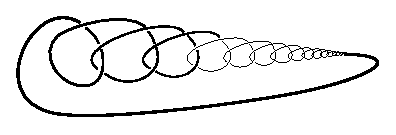
\includegraphics[scale=0.7]{images/wild}
	\caption{Un ejemplo de nudo salvaje.}
	\label{fig:wild}
\end{figure}

	 \index{Nudo!manso}
	 \index{Nudo!salvaje}
	 Para evitar patologías desagradables, consideraremos
	 únicamente nudos equivalentes a nudos dados por poligonales. Estos nudos se
	 llaman \textbf{nudos mansos}.  En la figura~\ref{fig:wild} mostramos un
	 ejemplo de nudo salvaje (no manso). Para nosotros, un \textbf{nudo} siempre
	 será un nudo manso. 
	 En la práctica, nuestros nudos poligonales tendrán tantos segmentos que
	 será casi imposible diferenciar a nuestra curva de una curva suave.  En
	 relación con esta observación, mencionamos el siguiente teorema:

    \begin{theorem}
        Un nudo parametrizado por longitud de arco y de clase $C^1$ es manso.
    \end{theorem}

    \begin{proof}
		La prueba de este resultado es muy técnica pero sólo utiliza conceptos
		básicos de cálculo avanzado.  Para una demostración completa referimos
		al apéndice I de \cite{MR0445489}.
    \end{proof}

	Para simplificar la notación, seremos un poco imprecisos a la hora
    de hablar de nudos.  Un nudo será una función inyectiva y
    continua $S^1\to\R^3$, su imagen o 
	una clase de equivalencia de tales funciones. 
	Por
    más extraño que parezca, esto no causará confusión alguna.

    \index{Diagrama de un nudo}
	Sea $K$ un nudo.  Consideremos la proyección de $K$ en el plano dada por
    \[
	\pi\colon(x,y,z)\mapsto(x,y).
	\]
	Un punto $p\in\pi(K)$ es un \textbf{punto
    múltiple} si $\pi^{-1}(p)$ contiene más de un punto de $K$. La
    \textbf{multiplicidad} de $p$ se define como el cardinal del conjunto
    $\pi^{-1}(p)\cap K$. Una proyección de $K$ en el plano se dice
    \textbf{genérica} si tiene las siguientes propiedades: 1) hay una cantidad finita de puntos
    de multiplicidad mayor a uno, 2) no hay puntos de multiplicidad mayor que 
    dos, y 3) no hay puntos dobles donde uno de los puntos es un vértice. La
    figura~\ref{fig:wrong_crossings} muestra algunos ejemplos de cruces no
    admitidos en una proyección genérica, el de la izquierda por ser un punto triple y los otros dos por presentar
    vértices. 
 
	\begin{figure}[ht]
        \centering
    	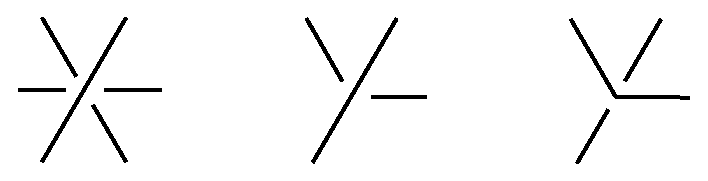
\includegraphics[scale=0.6]{images/wrongcrossings}
        \caption{Cruces no admitidos en el diagrama de un nudo dado por una
        poligonal.}
        \label{fig:wrong_crossings}
    \end{figure}
   
    Un \textbf{diagrama} de $K$ es una proyección genérica de $K$ en el plano
    donde en cada \textbf{cruce} (punto de multiplicidad dos) se puede
    distinguir qué segmento pasa por arriba y qué segmento pasa por debajo.
    Para ilustrar esta situación, el segmento que pasa por debajo se dibuja
    cortado.  Las componentes conexas del diagrama se llaman entonces
    \textbf{arcos}. Para diagramas de nudos orientados, agregaremos una flecha
    al diagrama que indique la orientación.

    \index{Nudo!trivial}
    Cualquier nudo equivalente a $S^1$ (visto como $S^1=\{(x,y,0)\in\R^3:x^2+y^2=1\}$) 
    será considerado como el \textbf{nudo
    trivial}.  En la práctica, no siempre es fácil reconocer la trivialidad de
    un nudo. En la figura~\ref{fig:trivial} vemos tres proyecciones distintas
    del nudo trivial. Una proyección aún más curiosa del nudo trivial puede
    verse en la figura~\ref{fig:thistlethwaite}.

    \begin{figure}[ht]
		\centering
    	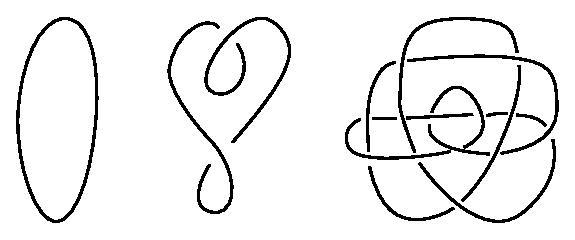
\includegraphics[scale=0.6]{images/unknots}
        \caption{Tres proyecciones del nudo trivial.}
        \label{fig:trivial}
	\end{figure}
	
	\begin{figure}
    	\centering
		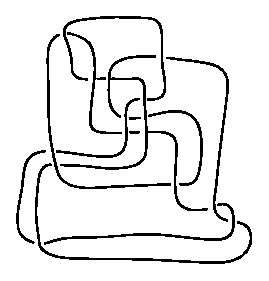
\includegraphics[scale=0.6]{images/thistlethwaite}
        \caption{Una proyección del nudo trivial descubierta por Thistlethwaite.}
        \label{fig:thistlethwaite}
    \end{figure}

    \label{block:reidemeister}
    \index{Reidemeister!movimientos de}
	En 1926 Reidemeister vislumbró una forma combinatoria de verificar si dos
	nudos son equivalentes. Básicamente, dos diagramas representarán al mismo
	nudo si y sólo si puede pasarse de un diagrama al otro mediante una
	sucesión finita de ciertas transformaciones, $\mathcal{R}_1$,
    $\mathcal{R}_2$ y $\mathcal{R}_3$, llamadas \textbf{movimientos de
	Reidemeister}.  Hay tres de estos movimientos:  el primero se muestra en la
	figura~\ref{fig:reidemeister1}, el segundo en la
	figura~\ref{fig:reidemeister2} y el tercero en la
	figura~\ref{fig:reidemeister3}. 

\begin{theorem}[Reidemeister]
	\index{Reidemeister!teorema de}
	\index{Teorema!de Reidemeister}
	Dos nudos son equivalentes si y sólo si sus diagramas están conectados
	por una sucesión finita de movimientos de Reidemeister.
\end{theorem}

\begin{proof}
	Para la demostración referimos a \cite[1.14]{MR3156509}.
\end{proof}

\begin{figure}[ht]
	\centering
    \begin{minipage}{0.3\textwidth}
		\centering
    	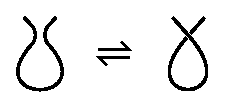
\includegraphics[width=0.6\textwidth]{images/reidemeisterI}
		\caption{$\mathcal{R}_1$}
		\label{fig:reidemeister1}
	\end{minipage}
	\begin{minipage}{0.3\textwidth}
		\centering
		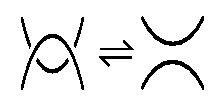
\includegraphics[width=0.6\textwidth]{images/reidemeisterII}
		\caption{$\mathcal{R}_2$}
		\label{fig:reidemeister2}
	\end{minipage}
	\begin{minipage}{0.3\textwidth}
		\centering
		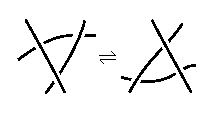
\includegraphics[width=0.7\textwidth]{images/reidemeisterIII}
		\caption{$\mathcal{R}_3$}
		\label{fig:reidemeister3}
	\end{minipage}
\end{figure}

El teorema de Reidemeister también puede utilizarse para nudos orientados si se
consideran todas las configuraciones posibles para los diagramas de las
figuras~\ref{fig:reidemeister1}, \ref{fig:reidemeister2} y \ref{fig:reidemeister3} con respecto a las
posibles orientaciones.  El teorema de Reidemeister es el núcleo de la teoría
combinatoria de nudos, ya que nos permite, por ejemplo, pensar que un nudo es
una clase de equivalencia de diagramas, donde dos diagramas son equivalentes si
y sólo si están conectados por una sucesión finita de movimientos de
Reidemeister.

\begin{example}
    El \textbf{nudo trébol} es quizá el nudo más famoso. Una representación
    paramétrica de la curva que da este nudo es 
    \begin{align*}
        &x=\sin(t)+2\sin(2t),\\
        &y=\cos(t)-2\cos(2t),\\
        &z=-\sin(3t).
    \end{align*}
	El nudo trébol, tal como lo vemos a la izquierda en la
	figura~\ref{fig:trefoil}, se denota por el símbolo $3_1$.  Queda como
	ejercicio demostrar que los dos nudos de la figura~\ref{fig:trefoil} son
	equivalentes.
\end{example}

\begin{example}
	\begin{figure}[ht]
		\centering
		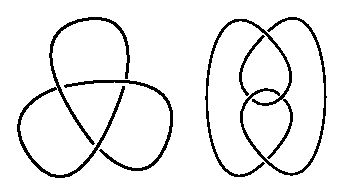
\includegraphics[scale=0.6]{images/trefoils}
		\caption{Dos proyecciones del nudo $3_1$.}
		\label{fig:trefoil}
	\end{figure}

    Otro nudo famoso es el nudo $4_1$ o \textbf{nudo ocho}. Una
    representación paramétrica para la curva que da este nudo es
	\begin{align*}
		x&=(2+\cos(2t))\cos(3t),\\
		y&=(2+\cos(2t))\sin(3t),\\
		z&=\sin(4t),
	\end{align*}
	y se puede ver una proyección en la figura~\ref{fig:4_1:unoriented}.
	\begin{figure}[ht]
		\centering
		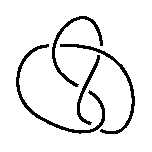
\includegraphics[scale=0.7]{images/4_1unoriented}
		\caption{El nudo $4_1$.}
		\label{fig:4_1:unoriented}
	\end{figure}
\end{example}

La \textbf{imagen especular} de un nudo se obtiene al aplicarle al nudo la
transformación $(x,y,z)\mapsto(x,y,-z)$.  En la figura
\ref{fig:trefoil_and_mirror} vemos el nudo $3_1$ y su imagen especular
$m(3_1)$. En el ejemplo \ref{exa:2cocycle:3_1andm(3_1)} demostraremos que los nudos
$3_1$ y $m(3_1)$ no son equivalentes. 
\begin{figure}[ht]
	\centering
		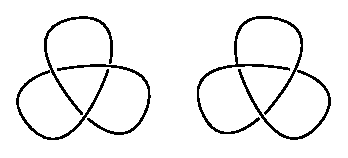
\includegraphics[scale=0.7]{images/trefoil_and_mirror}
		\caption{El nudo $3_1$ (derecha) y su imagen especular $m(3_1)$
		(izquierda).}
		\label{fig:trefoil_and_mirror}
\end{figure}
\begin{figure}[ht]
		\centering
		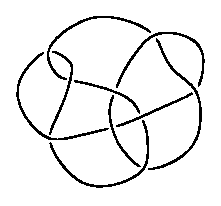
\includegraphics[scale=0.7]{images/9_32}
		\caption{El nudo $9_{32}$ es totalmente asimétrico.}
		\label{fig:9_32}
\end{figure}

Dos nudos orientados $K$ y $L$ serán equivalentes si existe una isotopía
entre $K$ y $L$ compatible las orientaciones.  Si $K$ es un nudo orientado, el
\textbf{reverso} $r(K)$ de $K$ es $K$ como conjunto pero con la orientación
opuesta. Los operadores $r$ y $m$ son involuciones en el espacio de nudos y
generan un grupo isomorfo a $\Z_2\times\Z_2$.

\begin{example}
	El nudo $3_1$ es equivalente al nudo $r(3_1)$. 
\end{example}

\begin{example}
	El nudo $4_1$ es
	\textbf{totalmente simétrico}, es decir: los nudos $4_1$, $m(4_1)$,
	$r(4_1)$ y $rm(4_1)$ son todos equivalentes.  
\end{example}

\begin{example}
	El nudo $9_{32}$ de la
	figura~\ref{fig:9_32} es \textbf{totalmente asimétrico}, es decir: los
	nudos $9_{32}$, $m(9_{32})$, $r(9_{32})$ y $rm(9_{32})$ son todos no
	equivalentes.
\end{example}

\section{Composición de nudos y nudos primos}
\label{section:composition}

Dados dos nudos orientados $K$ y $L$ podemos obtener un nuevo nudo con
el siguiente procedimiento: Quitamos un pedacito de arco de cada una de
las proyecciones de nuestros nudos y luego unimos los cuatro puntos
finales obtenidos con dos nuevos arcos (es importante que hagamos esto
sin agregar nuevos cruces) tal como muestra la figura~\ref{fig:composition}.
\begin{figure}[ht]
	\centering
	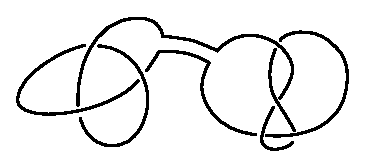
\includegraphics[scale=0.6]{images/composition}
	\caption{Composición de nudos.}
	\label{fig:composition}
\end{figure}

Esta operación se denomina \textbf{composición} de nudos. La composición de los
nudos $K$ y $L$ se denota por $K\#L$. No es difícil demostrar que la
composición de nudos es una operación asociativa y conmutativa y que el nudo
trivial es el neutro de esta operación.  Para más información referimos
a~\cite[\S1.2]{MR2079925}.  Un nudo no trivial es \textbf{primo} si no puede
descomponerse como la composición de otros nudos no triviales. Un nudo es
\textbf{compuesto} si no es primo.  El problema de determinar si un nudo dado
es primo es extremadamente difícil.  La figura \ref{fig:knots} contiene las
proyecciones de los primeros nudos primos (salvo reverso e imagen especular)
donde cada nudo tiene a lo sumo siete cruces. 
\begin{figure}[h]
	\centering
	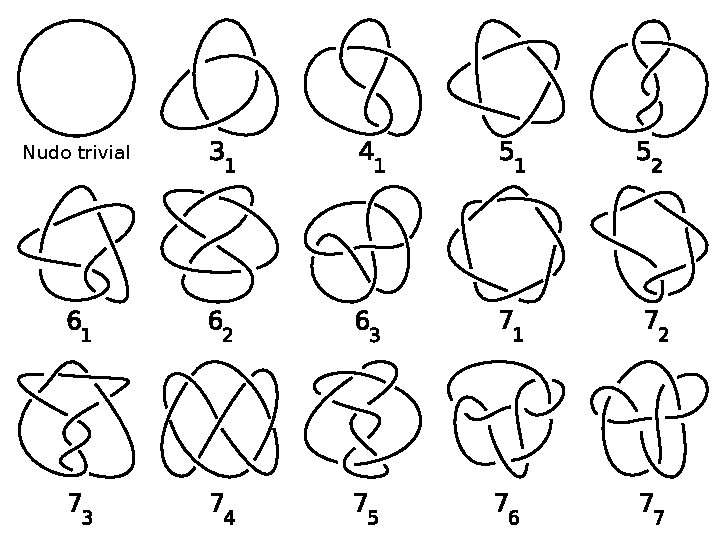
\includegraphics[scale=0.7]{images/knots}
	\caption{Algunos nudos primos.}
	\label{fig:knots}
\end{figure}

\begin{example}
	Consideremos el nudo que se forma al componer dos nudos $3_1$. Este nudo se
	conoce como el \textbf{nudo de la abuela} (o \emph{granny knot}, en
	inglés), se denota por $3_1\#3_1$, y se muestra a la izquierda en la
	figura~\ref{fig:granny_and_square}.  
\end{example}

\begin{example}
    El nudo compuesto formado por $3_1$ y su imagen especular $m(3_1)$ se conoce
    como el \textbf{nudo cuadrado} (o \emph{square knot}, en inglés), se denota
    por $3_1\#m(3_1)$, y se muestra a la derecha en la
    figura~\ref{fig:granny_and_square}. 
\end{example}
    
En los ejemplos \ref{exa:granny_vs_square:2} y \ref{exa:granny_vs_square:3}
demostraremos que el nudo de la abuela y el nudo cuadrado no son equivalentes.

\begin{figure}[ht]
	\centering
	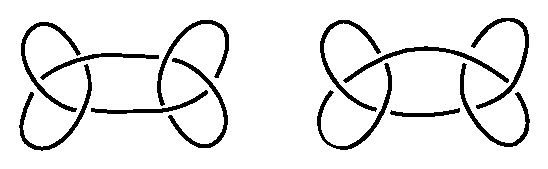
\includegraphics[scale=0.6]{images/grannyandsquare}
	\caption{El nudo de la abuela (izquierda) y el nudo cuadrado (derecha)
	no son equivalentes.}
	\label{fig:granny_and_square}
\end{figure}

Un teorema de H. Schubert establece que todo nudo puede expresarse en forma
única como la composición de nudos primos \cite[VII]{MR3156509}.  El género de
un nudo y las superficies de Seifert permiten demostrar que el nudo trivial no
puede escribirse como la composición de dos nudos no triviales, ver por ejemplo
\cite[\S4.3]{MR2079925}. Este resultado nos dice que no es posible hacer dos
nudos consecutivos en un pedacito de cuerda de forma tal que estos nudos se
cancelen mutuamente.  Como la demostración de este resultado es bastante
difícil, nos gustaría tener a mano una prueba más sencilla. Es por eso que
formulamos el siguiente problema:
\begin{quote}
	\textquestiondown Existe algún invariante sencillo que permita
	demostrar que el nudo trivial no puede escribirse como la composición
	de dos nudos no triviales? 
\end{quote}

Puede construirse un invariante de nudos a partir de la cantidad de cruces que
tienen los diagramas de un nudo.  Para ser más precisos, definiremos el
\textbf{número de cruces} $c(K)$ de un nudo $K$ como el menor número de cruces
que aparece en cualquier diagrama del nudo $K$. La siguiente conjetura lleva
abierta más de cien años y nos recuerda lo poco que sabemos del número $c(K)$,
ver~\cite[\S 3.3]{MR2079925} para más información.

\begin{conjecture}
	$c(K\#L)=c(K)+c(L)$. 
\end{conjecture}

\section{Coloraciones}
\label{section:coloreos}
\label{block:3coloring}
Supongamos que queremos mostrar que un cierto nudo no es trivial. \textquestiondown Qué
invariante sencillo podríamos obtener a partir de los tres movimientos de
Reidemeister? Responderemos esta pregunta al introducir la \textbf{coloración 
con tres colores}. Fijemos un conjunto de tres colores,
digamos $\{\textsf{rojo},\textsf{verde},\textsf{azul}\}$.  Una proyección
de un nudo es \textbf{coloreable con tres colores} si cada arco de la
proyección puede colorearse con uno de los tres colores de tal forma que en
cada cruce se vean los tres colores elegidos o únicamente uno de los tres. 

\begin{figure}[ht]
	\centering
    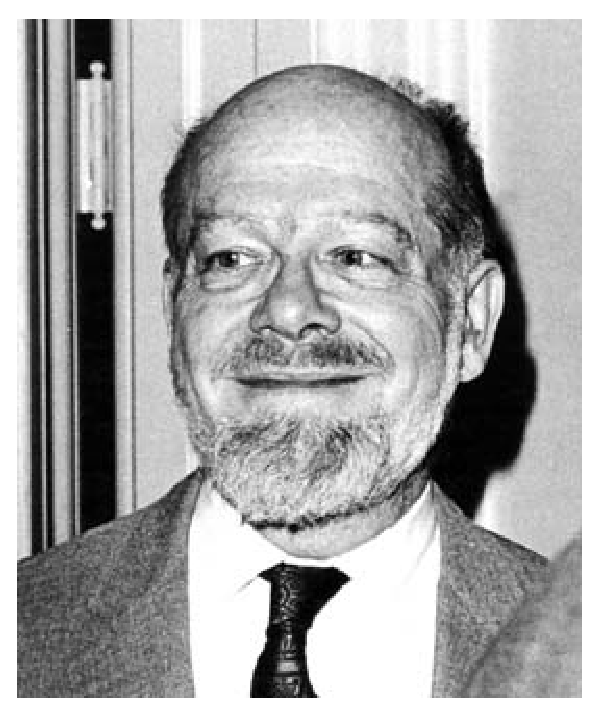
\includegraphics[width=30mm,height=36mm]{images/fox}
    \caption{Ralph Fox (1913--1973)}
\end{figure}

Podemos colorear cualquier nudo usando un sólo color. Esto nos da una coloración 
con tres colores que llamaremos \textbf{coloración trivial}. 

La cantidad de coloraciones con tres colores da un invariante de nudos. Este
resultado es un caso particular del teorema~\ref{theorem:fox} que veremos más
adelante. 

\begin{example}
    \label{exa:3colors}
    Las figuras~\ref{fig:3_1colors} 
	y~\ref{fig:4_1colors} nos muestran dos caras del mismo fenómeno: el nudo
	$3_1$ tiene coloraciones no triviales con tres colores y el nudo $4_1$ no.
	Vemos entonces que la coloración con tres colores nos permite distinguir el
	nudo $3_1$ del nudo trivial y del nudo $4_1$. Sin embargo, no nos permite
	determinar si el nudo $4_1$ es trivial. 
	\begin{figure}[ht]
		\begin{minipage}{0.45\textwidth}
			\centering
			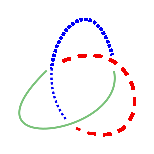
\includegraphics[scale=0.7]{images/3_1colors}
			\caption{El núdo $3_1$ coloreado con tres colores}
			\label{fig:3_1colors}
		\end{minipage}
		\begin{minipage}{0.45\textwidth}
			\centering
			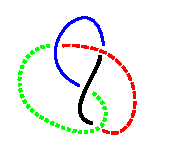
\includegraphics[scale=0.7]{images/4_1colors}
			\caption{El nudo $4_1$ puede colorearse con tres colores solamente de forma trivial.}
			\label{fig:4_1colors}
		\end{minipage}
	\end{figure}
\end{example}

Vamos a profundizar un poco en la idea de colorear con tres colores.
Supongamos que nuestros colores son los elementos de $\Z_3=\{0,1,2\}$ y que
$K$ es un nudo con $n$ cruces. Si etiquetamos los arcos del nudo $K$ con
los elementos de $\Z_3$ vemos que la condición que define coloraciones por
tres colores puede traducirse en términos de la compatibilidad de un
sistema de ecuaciones lineales que tiene una ecuación por cada cruce del
diagrama.  Para ser más precisos, la ecuación que corresponde al cruce de
la figura~\ref{fig:crossing} es $a+b+c=0$, donde $a,b,c\in\Z_3$.
Observemos que esta ecuación puede reescribirse como 
\begin{equation} 
	\label{eq:3colors}
	2a-b-c=0,
\end{equation}
donde el segmento que pasa por arriba está coloreado con el color $a$. 

Cada coloración del nudo $K$ será una solución del sistema de ecuaciones
formado por una ecuación análoga a \eqref{eq:3colors} por cada cruce. En particular, una
coloración no trivial será una solución que involucre todos los elementos
de $\Z_3$. 

\begin{figure}[ht]
	\centering
	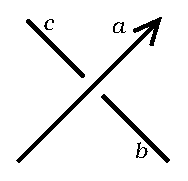
\includegraphics[scale=0.6]{images/crossing}
	\caption{Un cruce como este se colorea con la ecuación $2a-b-c=0$.}
	\label{fig:crossing}
\end{figure}

\begin{example}
	\label{exa:3_1:3colors}
	Si etiquetamos con $a,b,c\in\Z_3$ los arcos del diagrama del nudo $3_1$ que vemos 
	en la figura~\ref{fig:3_1colors}, el sistema
	de ecuaciones que resuelve el problema de la coloración con tres colores es el
	siguiente:
	\[
	\begin{cases}
		\begin{aligned}
			2a-b-c&=0,\\
			-a-b+2c&=0,\\
			-a+2b-c&=0.
		\end{aligned}
	\end{cases}
	\]
	La cantidad de coloraciones con tres colores del nudo $3_1$ es entonces la
	cantidad de vectores que tiene el núcleo de la \textbf{matriz de coloraciones}
	del nudo:
	\begin{equation*}
		C(3_1)=\begin{pmatrix}
		2 & -1 & -1\\
		-1 & -1 & 2\\
		-1 & 2 & -1
		\end{pmatrix}\in\Z_3^{3\times3}.
	\end{equation*}

    Como esta matriz tiene rango uno, el núcleo es un espacio vectorial (sobre
    $\Z_3$) de dimensión dos. Esto implica que el núcleo tiene nueve elementos,
    y por lo tanto el nudo $3_1$ tiene nueve coloraciones con tres colores (de los
    cuales seis son no triviales).
\end{example}

\label{block:fox}
En 1956 Fox definió una generalización de la coloración con tres colores.
Sea $p>2$ un número primo. Diremos que un nudo admite una \textbf{coloración de
Fox con $p$ colores} si cada arco puede etiquetarse con un elemento de 
$\Z_p=\{0,\dots,p-1\}$ de forma tal que en cada cruce como el que vemos
en la figura~\ref{fig:crossing} se cumple la ecuación
\[
	2a-b-c=0,
\]
donde $a,b,c\in\Z_p$.  Tal como se hizo en el
ejemplo~\ref{exa:3_1:3colors}, estudiar coloraciones de Fox con $p$ colores es
equivalente a estudiar el núcleo de la matriz de coloraciones vista como matriz
con coeficientes en $\Z_p$.

\begin{theorem}
    \label{theorem:fox}
	\index{Teorema!de Fox}
	\index{Fox!teorema de}
    Sea $p>2$ un número primo.  La cantidad de coloraciones de Fox con $p$ colores es
    un invariante de nudos. 

    \begin{proof}
        Fijemos un diagrama y una coloración de Fox del diagrama. Como vemos en la
        figura~\ref{fig:coloringR1}, la cantidad de coloraciones no se altera al aplicar el
        primer movimiento de Reidemeister ya que $b=2a-a=a$. 

        \begin{figure}[ht]
			\centering
	    	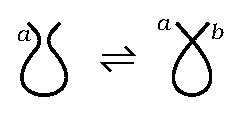
\includegraphics[scale=0.6]{images/coloringR1}
            \caption{La coloración de Fox da un invariante por el primer movimiento
            de Reidemeister pues $b=2a-a=a$.}
            \label{fig:coloringR1}
        \end{figure}

		La figura~\ref{fig:coloringR2} nos muestra que la cantidad de coloraciones de Fox 
		no se altera al aplicar el segundo movimiento de Reidemeister pues
		$c=2a-(2a-b)=b$.
        \begin{figure}[ht]
			\centering
	    	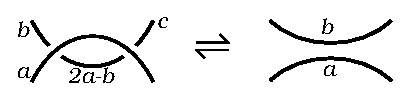
\includegraphics[scale=0.6]{images/coloringR2}
            \caption{La coloración de Fox da un invariante por el segundo movimiento
            de Reidemeister pues $c=2a-(2a-b)=b$.}
            \label{fig:coloringR2}
        \end{figure}

		La figura~\ref{fig:coloringR3} prueba que la cantidad de
		coloraciones es invariante bajo el tercer movimiento de Reidemeister
		pues $d=2a-(2b-c)$ y $d'=2(2a-b)-(2a-c)$ implican que $d=d'$.
		\begin{figure}[ht]
			\centering
				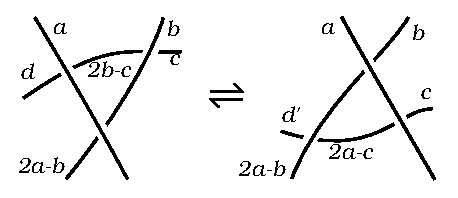
\includegraphics[scale=0.6]{images/coloringR3}
				\caption{La coloración de Fox da un invariante bajo el tercer movimiento
				de Reidemeister pues $d=d'$.}
				\label{fig:coloringR3}
		\end{figure}
		
        Hemos probado entonces que existe una biyección entre las coloraciones
        antes y después de aplicar los movimientos de Reidemeister. Luego, la
        cantidad de coloraciones de Fox es un invariante de nudos.
    \end{proof}
\end{theorem}

\begin{figure}[ht]
	\centering
	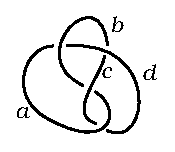
\includegraphics[scale=0.7]{images/labels4_1}
	\caption{Una coloración del nudo $4_1$.}
	\label{fig:labels4_1}
\end{figure}

\begin{example}
	\label{exa:4_1:colorings}
    Estudiemos algunas coloraciones del nudo $4_1$. Fijemos un número primo $p>2$.
    Si los arcos del nudo $4_1$ están etiquetados con
    $a,b,c,d\in\Z_p$ tal como vemos en la figura~\ref{fig:labels4_1}, el
    sistema de ecuaciones que resuelve el problema de la coloración de Fox con $p$
    colores es
    \begin{equation}
        \begin{cases}
            \begin{aligned}
                \label{eq:4_1:system}
                -a+2b-d&=0,\\
                -a-b+2c&=0,\\
                2a-c-d&=0,\\
                -b-c+2d&=0.
            \end{aligned}
        \end{cases}
    \end{equation}

	Como vimos en el ejemplo~\ref{exa:3colors}, la
	matriz asociada al sistema \eqref{eq:4_1:system} es lo que denominamos la
	matriz de coloraciones del nudo $4_1$:
	\begin{equation*}
		\label{eq:4_1:matrix}
		C(4_1)=\begin{pmatrix}
			-1 &  2 &  0 & -1\\
			-1 & -1 &  2 &  0\\
			2 &  0 & -1 & -1\\
			0 & -1 & -1 &  2
		\end{pmatrix}\in\Z_p^{4\times4}.
	\end{equation*}

	Un cálculo elemental nos muestra que 
	\[
	\dim\ker C(4_1)=\begin{cases}
		1 & \text{si $p=3$},\\
		2 & \text{si $p=5$}.
	\end{cases}
	\]
    Esto nos dice dos cosas: primero, que $4_1$ no puede colorearse de forma no
    trivial con tres colores; y segundo, que $4_1$ admite al menos una coloración
    de Fox no trivial con cinco colores. Luego, el nudo $4_1$ no es equivalente
    al nudo trivial. 
\end{example}

 \begin{exercise}
     Sean $p>2$ un número primo y $K$ un nudo con $n$ cruces. Pruebe que la
     cantidad de coloraciones de Fox con $p$ colores que tiene $K$ es $p^m$ para
     algún $m\leq n$.
 \end{exercise}

\begin{exercise}
    \label{exercise:colorings}
    El cuadro~\ref{tab:colorings} muestra cuáles de los nudos de la
    figura~\ref{fig:knots} admiten coloraciones de Fox no triviales para
    $p\in\{3,5,7,11,13,17\}$. \textquestiondown Qué conclusiones puede obtener? 

    \begin{table}[h]
		\centering
        \begin{tabular}{|c|c|c|c|c|c|c|}
            \hline 
            & $3$ & $5$ & $7$ & $11$ & $13$ & $17$\tabularnewline
            \hline 
            $3_{1}$ & $\surd$ &  &  &  &  & \tabularnewline
            \hline 
            $4_{1}$ &  & $\surd$ &  &  &  & \tabularnewline
            \hline 
            $5_{1}$ &  & $\surd$ &  &  &  & \tabularnewline
            \hline 
            $5_{2}$ &  &  & $\surd$ &  &  & \tabularnewline
            \hline 
            $6_{1}$ & $\surd$ &  &  &  &  & \tabularnewline
            \hline 
            $6_{2}$ &  &  &  & $\surd$ &  & \tabularnewline
            \hline 
            $6_{3}$ &  &  &  &  & $\surd$ & \tabularnewline
            \hline 
            $7_{1}$ &  &  & $\surd$ &  &  & \tabularnewline
            \hline 
            $7_{2}$ &  &  &  & $\surd$ &  & \tabularnewline
            \hline 
            $7_{3}$ &  &  &  &  & $\surd$ & \tabularnewline
            \hline 
            $7_{4}$ & $\surd$ & $\surd$ &  &  &  & \tabularnewline
            \hline 
            $7_{5}$ &  &  &  &  &  & $\surd$\tabularnewline
            \hline 
        \end{tabular}
        \caption{Algunas coloraciones de Fox para los nudos de la figura~\ref{fig:knots}.}
        \label{tab:colorings}
    \end{table}
\end{exercise}

\section{El grupo fundamental de un nudo}
\label{section:pi_1}

En esta sección definiremos el grupo fundamental de un nudo y mostraremos que
esta construcción da un buen invariante. Para una exposición detallada sobre
las nociones básicas respecto del grupo fundamental de un nudo referimos a
\cite{MR0445489}.

\begin{definition}
    \index{Grupo!fundamental de un nudo}
    El \textbf{grupo fundamental} $\pi_1(K)$ del nudo $K$ es el grupo de homotopía 
    $\pi_1(\R^3\setminus K)$. 
\end{definition}

\label{block:Wirtinger}
\begin{figure}
    \centering
	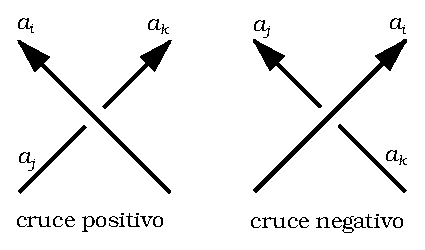
\includegraphics[scale=0.6]{images/crossings}
    \caption{Una orientación da dos tipos de
    cruce. En ambos casos, la relación de Wirtinger es $a_ia_ja_i^{-1}=a_k$.}
    \label{fig:crossings}
\end{figure}

    Veamos cómo calcular el grupo fundamental de un nudo.  Supongamos que $K$
    es un nudo con $n$ cruces.  Etiquetamos los arcos con las variables
    $a_1,a_2,a_3,\dots$ Como se ve en la figura~\ref{fig:crossings}, el
    diagrama tendrá dos tipos de cruce: cruces positivos y cruces negativos.
    Por cada cruce $\chi$ del diagrama como el que vemos en la
    figura~\ref{fig:crossings}, consideramos la \textbf{relación de Wirtinger}
    $r_\chi=1$, donde 
    $r_\chi = a_ia_ja_i^{-1}a_k^{-1}$. Como nos indice el siguiente teorema, 
	el grupo fundamental de
    $K$ es isomorfo al grupo dado por los generadores $a_1,a_2,a_3\dots$ y
    las relaciones de Wirtinger.  Esta presentación del grupo
    fundamental se conoce como la \textbf{presentación de Wirtinger}.

    \begin{theorem}[Wirtinger]
		\index{Teorema!de Wirtinger}
        \index{Wirtinger!teorema de}
        \index{Wirtinger!presentación de}
        Sea $K$ un nudo y supongamos que $K$ tiene una proyección con $n$ arcos
        y $m$ cruces. Entonces
        \begin{equation}
            \label{eq:knot_group}
            \pi_1(K)\simeq \langle a_1,a_2,\dots,a_n : r_1,r_2,\dots,r_m\rangle,
        \end{equation}
        donde las relaciones $r_1,\dots,r_m$ están dadas por las
        fórmulas de Wirtinger. La ecuación~\eqref{eq:knot_group}
        simboliza el cociente grupo libre en $a_1,\dots,a_n$ por el menor
        subgrupo normal que contiene a los elementos $r_1,\dots,r_m$. 
    \end{theorem}

    \begin{figure}[h]
		\centering
        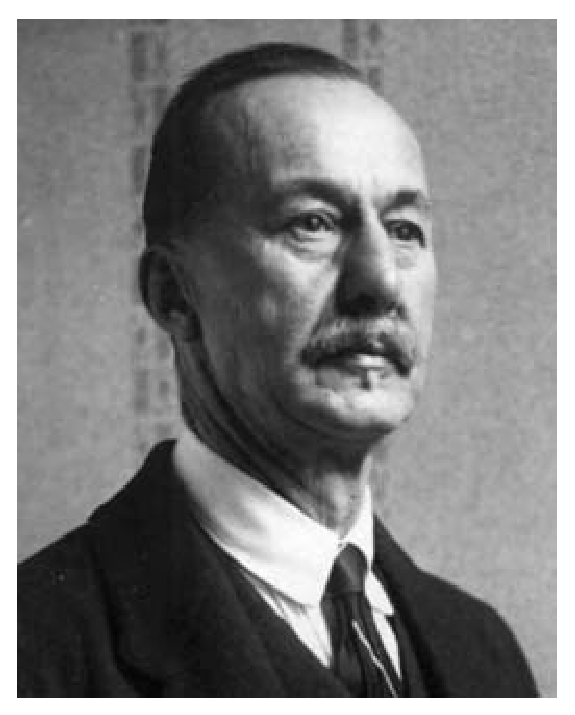
\includegraphics[width=30mm,height=36mm]{images/wirtinger}
        \caption{Wilhelm Wirtinger (1865--1945)}
    \end{figure}

\begin{exercise}
    Pruebe que el grupo fundamental del nudo trivial es isomorfo a $\Z$.
\end{exercise}

	\index{Teorema!de Dehn}
	\index{Dehn!teorema de}
	En 1915 Dehn demostró que el grupo fundamental permite detectar la
	trivialidad de un nudo. Más precisamente, el teorema de Dehn establece que
	un nudo es trivial si y sólo si el grupo fundamental del nudo es isomorfo a
	$\Z$. Es importante remarcar que, en general, es muy difícil determinar si
	un grupo finitamente presentado es isomorfo al grupo trivial. 

    \begin{figure}[h]
		\centering
        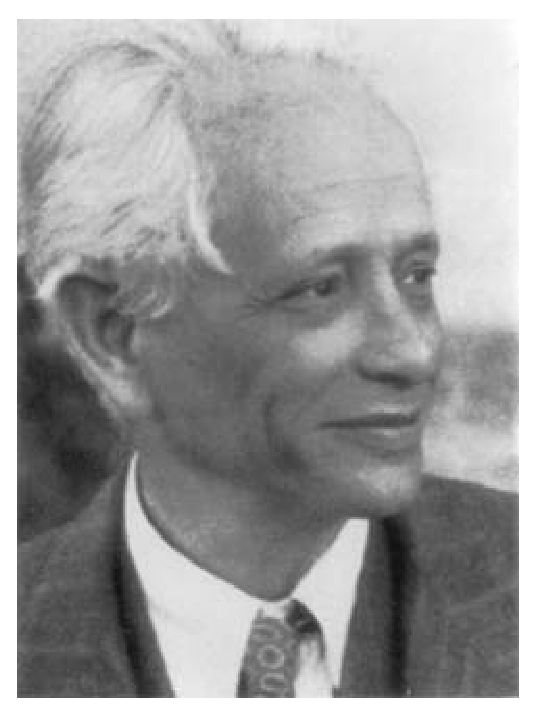
\includegraphics[width=30mm,height=36mm]{images/dehn}
        \caption{Max Dehn (1878--1952)}
    \end{figure}

\begin{example}
    \label{exa:3_1}
	\index{Nudo!$3_1$}
    Vamos a calcular el grupo fundamental del nudo $3_1$ que vemos en la
    figura~\ref{fig:oriented:3_1}. Las relaciones de Wirtinger son
    \begin{equation}
        a_1a_2a_1^{-1}=a_3,\quad
        a_2a_3a_2^{-1}=a_1,\quad
        a_3a_1a_3^{-1}=a_2,
    \end{equation}
    y entonces, 
    \[
        \pi_1(3_1)\simeq\langle a_1,a_2,a_3:\;
        a_1a_2a_1^{-1}=a_3,\;a_2a_3a_2^{-1}=a_1,\;a_3a_1a_3^{-1}=a_2\rangle.
    \]

    Vamos a utilizar el grupo $\pi_1(3_1)$ para dar otra demostración de la no
    trivialidad de $3_1$.  Como existe un morfismo sobreyectivo de grupos
    $\pi_1(3_1)\to\Sym_3$ tal que 
    \[
        a_1\mapsto(12),\quad
        a_2\mapsto(23),\quad
        a_3\mapsto(13),
    \]
    y el grupo simétrico $\Sym_3$ no es abeliano, se sigue que
    $\pi_1(3_1)$ es un grupo no abeliano. En particular
    $\pi_1(3_1)\not\simeq\Z$ y entonces el nudo $3_1$ no es equivalente al nudo
    trivial. 
\end{example}

\begin{exercise}
    Sea $n\in\N_{\geq2}$. Recordemos que el \textbf{grupo de trenzas} $\B_n$ se
    define como el grupo dado por los generadores $\sigma_1,\dots,\sigma_{n-1}$
    y las relaciones 
    \begin{align*}
        &\sigma_i\sigma_{i+1}\sigma_i=\sigma_{i+1}\sigma_i\sigma_{i+1} && \text{para todo $i\in\{1,\dots,n-2\}$},\\
        &\sigma_i\sigma_j=\sigma_j\sigma_i && \text{para todo par $i,j$ tal que $|i-j|>1$}.
    \end{align*}
    Pruebe que $\pi_1(3_1)\simeq\B_3$. 
\end{exercise}

\begin{figure}[ht]
	\centering
	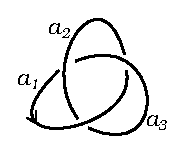
\includegraphics[scale=0.7]{images/3_1}
    \caption{El grupo fundamental de $3_1$ es isomorfo al grupo de trenzas $\B_3$.}
	\label{fig:oriented:3_1}
\end{figure}

\index{Gordon--Luecke!teorema de}
\index{Teorema!de Gordon--Luecke}
Tietze fue el primero en calcular el grupo fundamental del nudo $3_1$ en
1908. Ese mismo año conjeturó que dos nudos son equivalentes si y sólo si
sus complementos en $\R^3$ son homeomorfos. Muchos años después, en 1989,
Gordon y Luecke probaron esta afirmación \cite{MR965210}.  Como
consecuencia del teorema de Gordon y Luecke puede probarse que dos nudos
primos son equivalentes si y sólo si sus grupos fundamentales son
isomorfos. 

\begin{figure}[ht]
	\centering
    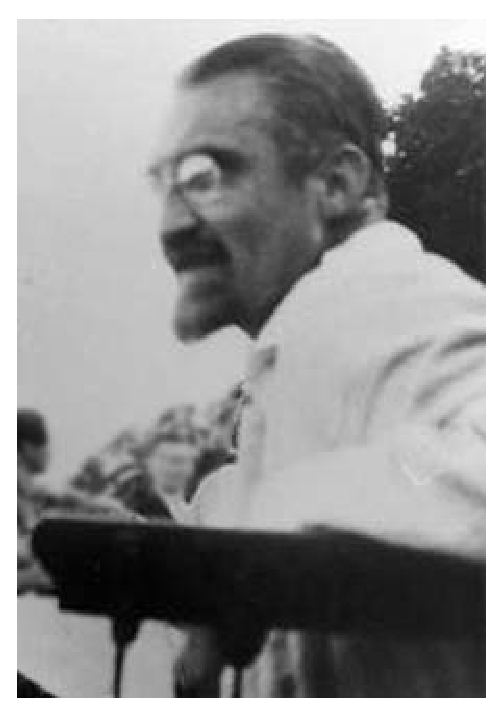
\includegraphics[width=30mm,height=36mm]{images/tietze}
    \caption{Heinrich Tietze (1880--1964)}
\end{figure}

\begin{example}
	\label{exa:4_1}
	\index{Nudo!$4_1$}
    Calculemos el grupo fundamental del nudo $4_1$ de la figura~\ref{fig:4_1}.
	El diagrama tiene dos cruces positivos y dos negativos. Las
	relaciones de Wirtinger son:
    \[
        a_4=a_1a_3a_1^{-1},\quad
        a_2=a_3a_1a_3^{-1},\quad
        a_1=a_2^{-1}a_4a_2,\quad           
        a_3=a_4^{-1}a_2a_4.
    \] 
    Puede demostrarse que 
    \[
    \pi_1(4_1)\simeq\langle x,y\mid xyx^{-1}yx=yxy^{-1}xy\rangle.
    \]

    Vamos a utilizar el grupo $\pi_1(4_1)$ para dar otra demostración de la no
    trivialidad del nudo~$4_1$. Consideremos el morfismo
    $\pi_1(4_1)\to\SL(2,\Z_3)$ dado por 
    \begin{align*}
        x\mapsto\begin{pmatrix}
            0 & 1\\
            2 & 1
        \end{pmatrix},\quad
        y\mapsto\begin{pmatrix}
            1 & 1\\
            2 & 0
        \end{pmatrix}.
    \end{align*}
    Como las imágenes de $x$ e $y$ no conmutan, se sigue que $\pi_1(4_1)$ no es
    abeliano. En particular $\pi_1(4_1)\not\simeq\Z$ y entonces $4_1$ no es el
    nudo trivial.
\end{example}

\begin{figure}[ht]
	\centering
	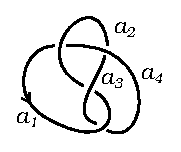
\includegraphics[scale=0.7]{images/4_1}
	\caption{El grupo fundamental de $4_1$ no es un grupo abeliano.}
	\label{fig:4_1}
\end{figure}

\begin{example}
    Ahora vamos a utilizar $\pi_1(4_1)$ para demostrar que los nudos $3_1$ y
    $4_1$ no son equivalentes.  Por lo visto en el ejemplo~\ref{exa:3_1}, si
    los grupos $\pi_1(4_1)$ y $\pi_1(3_1)$ fueran isomorfos, existiría un
    epimorfismo $\pi_1(4_1)\to\Sym_3$. Sin embargo, un cálculo directo muestra
    que ningún morfismo $\pi_1(4_1)\to\Sym_3$ es sobreyectivo.
\end{example}

\begin{exercise}
    \index{Nudo!de la abuela}
    \index{Nudo!cuadrado}
    \label{exercise:granny_and_square}
	En la figura~\ref{fig:granny_and_square} vimos dos nudos compuestos: el
	nudo de la abuela y el nudo cuadrado.  Pruebe que estos nudos tienen grupos
	fundamentales isomorfos. 
\end{exercise}

Como veremos más adelante, el nudo de la abuela y el nudo cuadrado no son
equivalentes. Luego, el grupo fundamental de un nudo es un buen invariante
pero no es infalible, es decir: existen nudos no equivalentes con grupos
fundamentales isomorfos. 

\section{Quandles}
\label{section:quandles}

Sabemos que gracias a los movimientos de Reidermeister el problema de
distinguir nudos puede formularse en términos de combinatoria. En esta
sección vamos a definir el quandle fundamental de un nudo y vamos a probar que
es un invariante que generaliza al grupo fundamental y a los invariantes por
coloraciones.

Los quandles son estructuras algebraicas que modelan la conjugación en un
grupo. La primera aparición de una familia de quandles se produjo en 1943
cuando Mituhisa Takasaki introdujo los quandles involutivos --los llamó
\emph{keis}-- con el fin de entender las reflexiones. En 1959, los matemáticos
ingleses John Conway y Gavil Wraith, después de un interesante intercambio
de cartas e ideas, definieron los \emph{wracks}. La idea de Conway y Wraith
es que un wrack (hoy llamado simplemente \emph{pecio} o \emph{rack} en
inglés) es esencialmente lo que queda de un grupo una vez que uno olvida la
multiplicación y se preocupa únicamente por la conjugación.  En 1982 Joyce
introdujo los \emph{quandles} con el fin de producir invariantes de nudos.
Inspirado en la presentación de Wirtinger del grupo fundamental de un nudo,
Joyce construyó el \emph{quandle fundamental} de un nudo y probó que esta
construcción da un buen invariante de nudos no orientados.  Ese mismo año,
y de forma independiente, Sergei Matveev también introdujo los quandles
--que él llamó \emph{grupoides distributivos}-- y probó un resultado similar
al de Joyce.  En 1988, para estudiar ciertos aspectos de la teoría de
singularidades de curvas, el matemático alemán Egbert Brieskorn introdujo
una estructura equivalente a la de Conway y Wraith: los \emph{automorphic
sets}. 
    \begin{figure}[h]
		\centering
        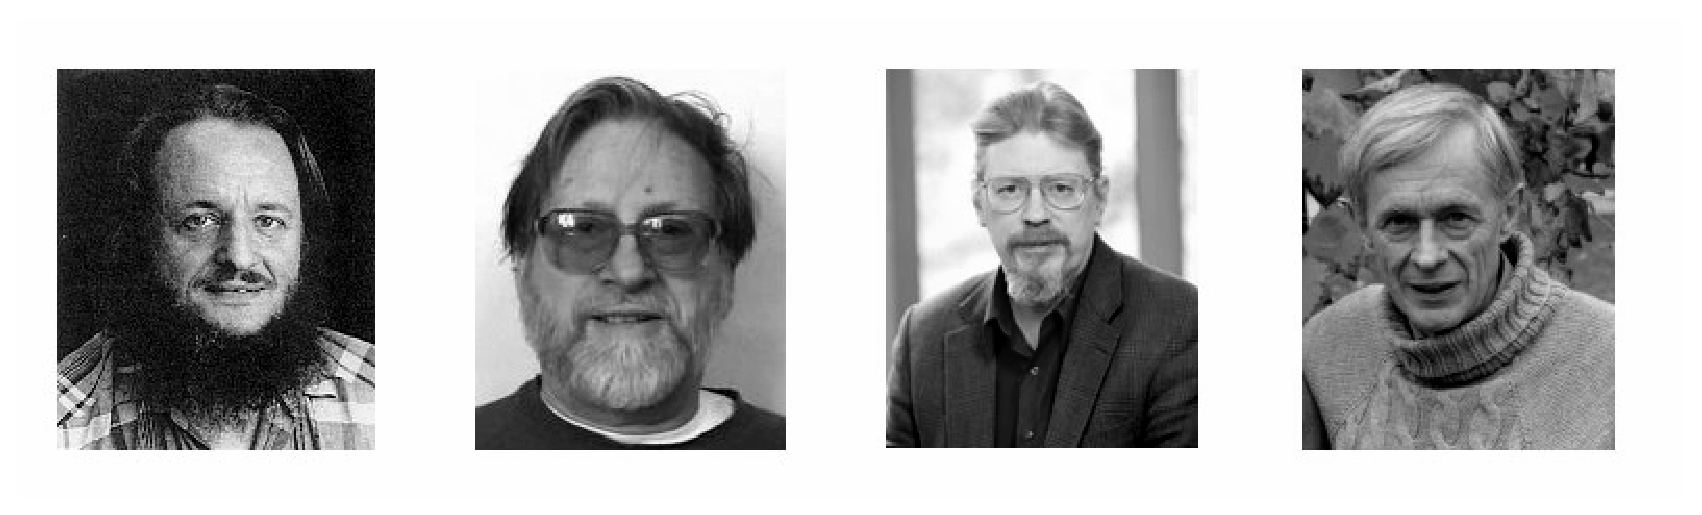
\includegraphics[scale=0.4]{images/cwjb}
        \caption{Algunos de los fundadores de la teoría de quandles. De
        izquierda a derecha: John Conway, Gavin Wraith, David Joyce, Egbert Brieskorn.}
    \end{figure}

	\begin{definition}
		\index{Quandle}
		\label{block:quandle}
		Un \textbf{quandle} es un par $(X,\triangleright)$, donde $X$ es un
		conjunto no vacío con una operación binaria $X\times X\to X$,
		$(x,y)\mapsto x\triangleright y$, tal que
		\begin{align}
			& \varphi_x\colon X\to X,\;y\mapsto x\triangleright y\text{ es biyectiva},&&\text{ para todo $x\in X$},\\
			& x\triangleright (y\triangleright z)=(x\triangleright y)\triangleright (x\triangleright z) && \text{para todo $x,y,z\in X$},\\
			& x\triangleright x=x && \text{para todo $x\in X$}.
		\end{align}
	\end{definition}

	Utilizaremos la siguiente notación: $x\triangleright^{-1}
	y=\varphi_x^{-1}(y)$. 

\begin{example}
    Si $G$ es un grupo, entonces $G$ es un quandle con $x\triangleright y=xyx^{-1}$ para todo $x,y\in X$.  
\end{example}

	El artículo de Joyce utiliza una definición de quandle levemente distinta a
	la que damos en este artículo, ya que Joyce usa acciones a derecha y no
	acciones a izquierda. 

	\begin{definition}
		Sean $X$ e $Y$ dos quandles. Una función $f\colon X\to Y$ es un
		\textbf{morfismo} de quandles si $f(x\triangleright x')=f(x)\triangleright
		f(x')$ para todo $x,x'\in X$.
	\end{definition}

\begin{example}
    \index{Quandle!trivial} Sea $X$ un conjunto no vacío. Entonces $X$ es un
    quandle con $x\triangleright y=y$ para todo $x,y\in X$. Este quandle se
    denomina \textbf{quandle trivial} sobre $X$.
\end{example}

\begin{example}
    \index{Quandle!de conjugación}
    Sean $G$ un grupo y $X$ una clase de conjugación de $G$. Entonces $X$ es un
    quandle con $x\triangleright y=xyx^{-1}$ para todo $x,y\in X$.  El quandle
    asociado a la clase de conjugación de $g$ en $G$ se llama \textbf{quandle
	de conjugación} asociado a (la clase de) $g$ en $G$.
\end{example}

\begin{exercise}
    Si $X$ es un quandle de conjugación entonces 
    \begin{equation}
        \label{eq:crossed_set}
        x\triangleright y=y\Longleftrightarrow y\triangleright x=x\quad\text{para todo $x,y\in X$}.
    \end{equation}
    Encuentre un quandle de tres elementos que no cumpla con la
    condición~\eqref{eq:crossed_set}. 
\end{exercise}

\begin{exercise}
    \index{Quandle!diedral}
	Sea $n\in\N_{\geq3}$. Pruebe que $\Z_n$ es un quandle con 
    $x\triangleright y=2x-y$ para todo $x,y\in\Z_n$. Este quandle se denomina
    \textbf{quandle diedral} y se denota por $\D_n$. 
\end{exercise}

\begin{example}
    \label{block:alexander}
    Sea $M$ un $\Z[t,t^{-1}]$-módulo a izquierda.  Definimos el \textbf{quandle
    de Alexander} sobre $M$ como el quandle dado por 
    \begin{align}
        \label{eq:alexander}
        x\triangleright y=(1-t)x+t y\qquad\text{para todo $x,y\in M$.}
    \end{align}

    Demostremos que la acción \eqref{eq:alexander} define una estructura de
    quandle sobre $M$. Es evidente que para cada $x\in M$ la función
    $\varphi_x\colon y\mapsto (1-t)x+ty$ es inversible y la inversa
    $\varphi_x^{-1}$ está dada por $y\mapsto (1-t^{-1})x+t^{-1}y$.
    Además $x\triangleright x=x$ para todo $x\in X$. Para demostrar la
    distributividad, tomamos $x,y,z\in M$ y calculamos
    \begin{align*}
        (x\triangleright y)\triangleright (x\triangleright z) &= \left( (1-t)x+ty \right)\triangleright \left( (1-t)x+tz \right)\\
        &= (1-t)\left( (1-t)x+t y \right)+t\left( (1-t)x+t z \right)\\
        &= (1-t)x+t(1-t)y+t^2z\\
        &= (1-t)x+t(y\triangleright z)\\
        &= x\triangleright(y\triangleright z).
    \end{align*}

    \begin{figure}[h]
		\centering
        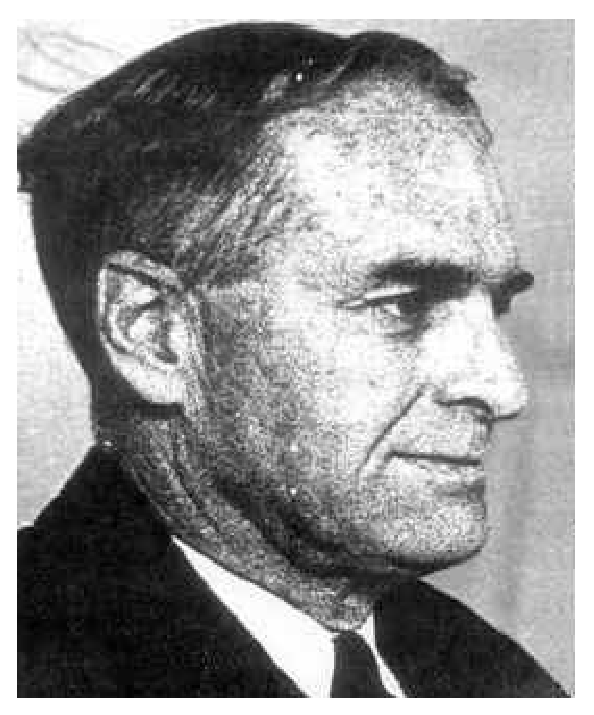
\includegraphics[width=30mm,height=36mm]{images/alexander}
        \caption{James Alexander (1888--1971)}
    \end{figure}
\end{example}

	Veamos un caso particular de la contrucción del quandle de Alexander. 

\begin{example}
    Sea $\F_q$ el cuerpo de $q$ elementos, donde $q$ es una potencia de un
    número primo. Para cada $\alpha\in\F_q\setminus\{0\}$ definimos el
    \textbf{quandle de Alexander} de tipo $(q,\alpha)$ como el quandle sobre 
    $\F_q$ dado por 
    $x\triangleright y=(1-\alpha)x+\alpha y$ para todo $x,y\in\F_q$.
\end{example}

\begin{exercise}
	Pruebe que el quandle de conjugación asociado a la clase de $(123)$ en
	$\Alt_4$ es isomorfo a un quandle de Alexander.
\end{exercise}

\label{block:fundamental_quandle}
    \index{Quandle!fundamental de un nudo}
    Así como puede calcularse el grupo fundamental de un nudo gracias a la
    presentación de Wirtinger, es posible considerar el quandle fundamental de
    un nudo. Supongamos que $K$ es un nudo con $n$ arcos y $m$
    cruces.  Como hicimos con las relaciones de Wirtinger, etiquetamos los arcos de la
    proyección con las variables $a_1,a_2,a_3\dots$ En cada cruce $\chi$ como
    el que vemos en la figura \ref{fig:crossings} consideramos la relación
    \begin{equation}
        \label{eq:Joyce}
        r_\chi:a_i\triangleright a_j=a_k.          
    \end{equation}

\begin{definition}
    El \textbf{quandle fundamental} del nudo $K$ es el quandle 
    \[
        Q(K)=\langle a_1,a_2,\dots,a_n:r_1,\dots,r_m\rangle,
    \]
    donde las relaciones $r_1,\dots,r_m$ están dadas por las fórmulas
    \eqref{eq:Joyce}.
\end{definition}

\begin{example}
    \label{exa:3_1:fundamental_quandle}
    El quandle fundamental del nudo $3_1$ de la 
    figura~\ref{fig:oriented:3_1} es 
    \begin{equation}
        \label{eq:3_1:fundamental_quandle}
        Q(3_1)=\langle a_1,a_2,a_3:
		a_1\triangleright a_2=a_3,\; 
		a_2\triangleright a_3=a_1,\;
		a_3\triangleright a_1=a_2\rangle.
    \end{equation}
\end{example}
	
\begin{example}
    \label{exa:4_1:fundamental_quandle}
    En el ejemplo~\ref{exa:4_1} calculamos el grupo fundamental del nudo $4_1$.
    El quandle fundamental del nudo $4_1$ de la figura~\ref{fig:4_1} es 
    \begin{multline}
        \label{eq:4_1:fundamental_quandle}
        Q(4_1)=\langle a_1,\dots,a_4:
        a_1\triangleright a_3=a_4,\; 
		a_3\triangleright a_1=a_2,\;
        a_2\triangleright a_1=a_4,\;
        a_4\triangleright a_3=a_2\rangle.
    \end{multline}
    Observemos que las dos primeras relaciones corresponden a cruces positivos
    y las dos últimas a cruces negativos.  
\end{example}


	\label{block:quandle_proof} No es difícil demostrar que el quandle
	fundamental de un nudo queda invariante por los movimientos de
	Reidemeister. La demostración es apenas más complicada que la del
	teorema~\ref{theorem:fox}. La diferencia está en que ahora habrá más diagramas
	de Reidemeister para verificar pues deben considerarse todas las
	configuraciones posibles con respecto a la orientación del nudo. 
    Para el primer movimiento de Reidemeister deben verificarse los diagramas de
    la figura~\ref{fig:oriented_R1}.
    Las posibles configuraciones que pueden aparecer en el segundo movimiento de
    Reidemeister se muestran en la figura~\ref{fig:oriented_R2}. 

    \begin{figure}[ht]
	%	\begin{minipage}{0.5\textwidth}
		\centering
        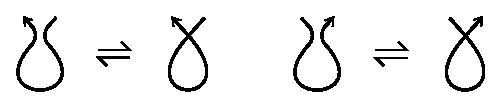
\includegraphics[scale=0.6]{images/oriented_R1}
        \caption{Las configuraciones posibles en el primer movimiento de Reidemeister.}
        \label{fig:oriented_R1}
    \end{figure}
    %\end{minipage}
	%\begin{minipage}{0.5\textwidth}
	\begin{figure}[ht]
		\centering
        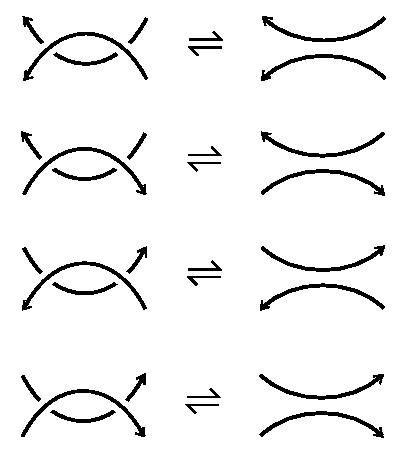
\includegraphics[scale=0.6]{images/oriented_R2}
        \caption{Las cuatro configuraciones posibles en el segundo movimiento de Reidemeister.}
        \label{fig:oriented_R2}
    %\end{minipage}
    \end{figure}

	Finalmente, para el tercer movimiento hay ocho posibles diagramas. Por
	ejemplo, la condición a verificar en la figura~\ref{fig:oriented_R3a} es
    \begin{equation*}
        a\triangleright^{-1}(b\triangleright c)=(a\triangleright^{-1}b)\triangleright(a\triangleright^{-1}c),
    \end{equation*}
    que es consecuencia de la definición~\ref{block:quandle}.

    \begin{figure}[h]
		\centering
        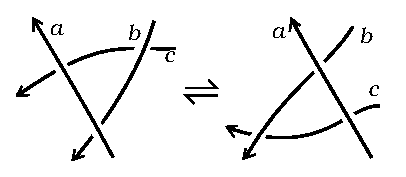
\includegraphics[scale=0.6]{images/oriented_R3a}
        \caption{Una de las configuraciones posibles para el tercer movimiento de Reidemeister.}
        \label{fig:oriented_R3a}
    \end{figure}

	\begin{theorem}[Matveev]
	\index{Teorema!de Matveev}
	\index{Matveev!teorema de}
		Si $K$ y $L$ son dos nudos, entonces 
		$Q(K)\simeq Q(L)$ si y sólo si $L=K$ o $L=rm(K)$, donde $rm(K)=r(m(K))$ es el reverso de la imagen
		especular de $K$.
	\end{theorem}

	\begin{proof}
	Para la demostración referimos a \cite{MR672410}.
	\end{proof}

	\index{Grupo!envolvente de un quandle}
	Sea $X$ un quandle. El \textbf{grupo envolvente} de $X$ es el grupo
	\[
		G_X=F_X/\langle xy=(x\triangleright y)x,\;x,y\in X\rangle,
	\]
	donde $F_X$ es el grupo libre con base en los elementos de $X$.

	\begin{theorem}[Joyce]
	\index{Teorema!de Joyce}
	\index{Joyce!teorema de}
		$G_{Q(K)}\simeq\pi_1(K)$ para todo nudo $K$. 
	\end{theorem}

	\begin{proof}
		La demostración aparece en~\cite{MR638121}.
	\end{proof}

	Es importante remarcar que el problema de determinar si dos grupos o dos
	quandles son isomorfos es, en general, muy difícil de resolver.

\section{Ejemplos de quandle fundamentales}

	\label{block:5_1:fundamental_quandle}
	\label{block:5_2:fundamental_quandle}
	\index{Nudo!$5_1$}
	\index{Nudo!$5_2$}

    Consideremos el nudo $5_1$ de la figura~\ref{fig:5_1}. Todos los cruces del
    diagrama son positivos y el quandle fundamental de $5_1$ es
	\begin{multline}
        \label{eq:5_1}
        Q(5_1)=\langle a_1,\dots a_5:
		a_1\triangleright a_3=a_4,\;
        a_4\triangleright a_1=a_2,\;
        a_2\triangleright a_4=a_5,\\
        a_5\triangleright a_2=a_3,\; 
        a_3\triangleright a_5=a_1\rangle.
    \end{multline}

    Consideremos ahora el nudo $5_2$ de la figura~\ref{fig:5_2}. Todos los
    cruces del diagrama son positivos y entonces el quandle fundamental
    $Q(5_2)$ es
	\begin{multline}
        Q(5_2)=\langle a_1,\dots a_5:
		a_1\triangleright a_4=a_5,\;
		a_4\triangleright a_1=a_2,\;
		a_2\triangleright a_3=a_4,\\
		a_5\triangleright a_2=a_3,\;
		a_3\triangleright a_5=a_1\rangle.
	\end{multline}

	\begin{figure}[ht]
		\centering
		\begin{minipage}{0.4\textwidth}
			\centering
			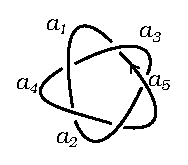
\includegraphics[scale=0.7]{images/5_1}
			\caption{$5_1$}
			\label{fig:5_1}
		\end{minipage}
		\begin{minipage}{0.4\textwidth}
			\centering
			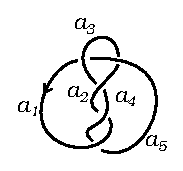
\includegraphics[scale=0.7]{images/5_2}
			\caption{$5_2$}
			\label{fig:5_2}
		\end{minipage}
	\end{figure}

	\label{block:Q(6_1):fundamental_quandle}
	\label{block:Q(6_2):fundamental_quandle}
	\label{block:Q(6_3):fundamental_quandle}
	\index{Nudo!$6_1$}
    El quandle fundamental $Q(6_1)$ del nudo $6_1$ de la figura~\ref{fig:6_1} es
	\begin{multline}
		Q(6_1)=\langle a_1,\dots,a_6:
		a_1\triangleright a_4=a_3,\;
		a_3\triangleright a_2=a_1,\;
		a_2\triangleright a_5=a_6,\\
		a_5\triangleright a_2=a_3,\;
		a_4\triangleright a_1=a_6,\;
		a_6\triangleright a_5=a_4\rangle,
	\end{multline}
    donde las ecuaciones $a_2\triangleright a_5=a_6$ y $a_5\triangleright
    a_2=a_3$ corresponden a los únicos cruces positivos. 
	\index{Nudo!$6_2$}
    El quandle fundamental del nudo $6_2$ tal como lo vemos en la
    figura~\ref{fig:6_2} es
	\begin{multline}
		Q(6_2)=\langle a_1,\dots,a_6:
		a_1\triangleright a_4=a_5,\;
		a_5\triangleright a_3=a_2,\;
		a_2\triangleright a_6=a_5,\\
		a_6\triangleright a_3=a_4,\;
		a_3\triangleright a_1=a_2,\;
		a_4\triangleright a_6=a_1\rangle,
	\end{multline}
    donde las ecuaciones $a_5\triangleright a_3=a_2$ y $a_2\triangleright
    a_6=a_5$ corresponden a los únicos cruces positivos del diagrama.  
	\index{Nudo!$6_3$}
    Por último, el quandle fundamental del nudo $6_3$ de la figura~\ref{fig:6_3} es 
	\begin{multline}
		\label{eq:Q(6_3)}
		Q(6_3)=\langle a_1,\dots,a_6:
			a_1\triangleright a_5=a_4,\;
			a_5\triangleright a_2=a_1,\;
			a_2\triangleright a_3=a_4,\\
			a_6\triangleright a_2=a_3,\;
			a_3\triangleright a_6=a_1,\;
			a_4\triangleright a_6=a_5\rangle,
	\end{multline}
    donde las ecuaciones $a_2\triangleright a_3=a_4$, $a_6\triangleright
    a_2=a_3$ y $a_3\triangleright a_6=a_1$ corresponden a los únicos cruces
    positivos del diagrama. 

\begin{figure}[ht]
		\centering
		\begin{minipage}{0.4\textwidth}
			\centering
		    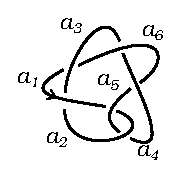
\includegraphics[scale=0.7]{images/6_1}
			\caption{$6_1$}
			\label{fig:6_1}
		\end{minipage}
		\begin{minipage}{0.4\textwidth}
			\centering
		    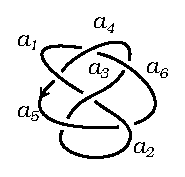
\includegraphics[scale=0.7]{images/6_2}
			\caption{$6_2$}
			\label{fig:6_2}
		\end{minipage}
		\begin{minipage}{0.4\textwidth}
			\centering
		    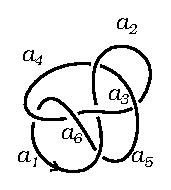
\includegraphics[scale=0.7]{images/6_3}
			\caption{$6_3$}
			\label{fig:6_3}
		\end{minipage}
	\end{figure}

	\label{block:Q(7_1):fundamental_quandle}
	\label{block:Q(7_2):fundamental_quandle}
	\label{block:Q(7_3):fundamental_quandle}
	\label{block:Q(7_4):fundamental_quandle}
	\label{block:Q(7_5):fundamental_quandle}
	\label{block:Q(7_6):fundamental_quandle}
	\label{block:Q(7_7):fundamental_quandle}
	\index{Nudo!$7_1$}
    Presentemos los quandles fundamentales de los nudos de la
    figuras~\ref{fig:7_1}--\ref{fig:7_5}. Un cálculo directo muestra que
	\begin{multline}
		Q(7_1)=\langle a_1,\dots,a_7:
		a_1\triangleright a_4=a_5,\;
		a_5\triangleright a_1=a_2,\;
		a_2\triangleright a_5=a_6,\\
		a_6\triangleright a_2=a_3,\;
		a_3\triangleright a_6=a_7,\;
		a_7\triangleright a_3=a_4,\;
		a_4\triangleright a_7=a_1\rangle,
	\end{multline}
    donde todos los cruces involucrados son positivos. 
	\index{Nudo!$7_2$}
	Similarmente, 
	\begin{multline}
		Q(7_2)=\langle a_1,\dots,a_7:
		a_1\triangleright a_4=a_3,\;
		a_3\triangleright a_2=a_1,\;
		a_2\triangleright a_6=a_5,\\
		a_5\triangleright a_7=a_6,\;
		a_7\triangleright a_5=a_4,\;
		a_4\triangleright a_1=a_7,\;
		a_6\triangleright a_3=a_2\rangle,
	\end{multline}
    donde todos los cruces son negativos. 

	\begin{figure}[ht]
		\centering
		\begin{minipage}{0.4\textwidth}
			\centering
			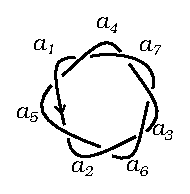
\includegraphics[scale=0.7]{images/7_1}
			\caption{$7_1$}
			\label{fig:7_1}

		\end{minipage}
		\begin{minipage}{0.4\textwidth}
			\centering
			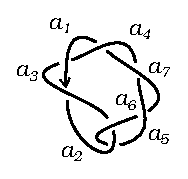
\includegraphics[scale=0.7]{images/7_2}
			\caption{$7_2$}
			\label{fig:7_2}

% 		\end{minipage}
% 		\begin{minipage}{0.4\textwidth}
% 			\centering
% 			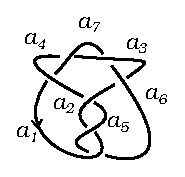
\includegraphics[scale=0.7]{images/7_3}
% 			\caption{$7_3$}
% 			\label{fig:7_3}
% 		\end{minipage}
% 		\begin{minipage}{0.4\textwidth}
% 			\centering
% 	    	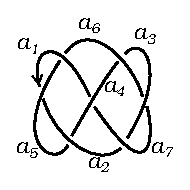
\includegraphics[scale=0.7]{images/7_4}
% 			\caption{$7_4$}
% 			\label{fig:7_4}
 		\end{minipage}
 	\end{figure}


	\index{Nudo!$7_3$}
	Para el nudo $7_3$ tenemos
	\begin{multline}
		Q(7_3)=\langle a_1,\dots,a_7:
		a_1\triangleright a_5=a_6,\;
		a_5\triangleright a_1=a_2,\;
		a_2\triangleright a_4=a_5,\\
		a_6\triangleright a_2=a_3,\;
		a_3\triangleright a_6=a_7,\;
		a_7\triangleright a_3=a_4,\;
		a_4\triangleright a_7=a_1\rangle,
	\end{multline}
    donde todos los cruces son positivos. 
	\index{Nudo!$7_4$}
    Para el nudo $7_4$ se tiene
	\begin{multline}
		Q(7_4)=\langle a_1,\dots,a_7:
		a_5\triangleright a_1=a_2,\;
		a_2\triangleright a_4=a_5,\;
		a_4\triangleright a_1=a_7,\\
		a_6\triangleright a_3=a_4,\;
		a_3\triangleright a_6=a_7,\;
		a_7\triangleright a_2=a_3,\;
		a_1\triangleright a_5=a_6\rangle,
	\end{multline}
    donde la ecuación $a_4\triangleright a_1=a_7$ corresponde al único cruce
    negativo que tiene el diagrama. 
	
	\begin{figure}[ht]
		\centering
		\begin{minipage}{0.4\textwidth}
			\centering
			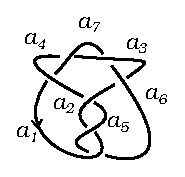
\includegraphics[scale=0.7]{images/7_3}
			\caption{$7_3$}
			\label{fig:7_3}
		\end{minipage}
		\begin{minipage}{0.4\textwidth}
			\centering
	    	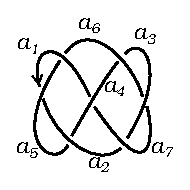
\includegraphics[scale=0.7]{images/7_4}
			\caption{$7_4$}
			\label{fig:7_4}
		\end{minipage}
	\end{figure}
	
	\index{Nudo!$7_5$}
	Para el nudo $7_5$ se obtiene 
	\begin{multline}
		Q(7_5)=\langle a_1,\dots,a_7:
		a_1\triangleright a_4=a_3,\;
		a_5\triangleright a_2=a_1,\;
		a_2\triangleright a_6=a_5,\\
		a_7\triangleright a_3=a_2,\;
		a_3\triangleright a_1=a_7,\;
		a_4\triangleright a_7=a_6,\;
		a_6\triangleright a_4=a_5\rangle,
	\end{multline}
    donde la ecuación $a_6\triangleright a_4=a_5$ corresponde al único cruce
    negativo del diagrama.  
	\index{Nudo!$7_6$}
	Para el nudo $7_6$ tenemos
	\begin{multline}
		Q(7_6)=\langle a_1,\dots,a_7:
		a_6\triangleright a_2=a_1,\;
		a_4\triangleright a_3=a_2,\;
		a_2\triangleright a_6=a_5,\\
		a_3\triangleright a_1=a_7,\;
		a_1\triangleright a_2=a_3,\;
		a_7\triangleright a_4=a_5,\;
		a_5\triangleright a_6=a_7\rangle,
	\end{multline}
    donde las relaciones $a_1\triangleright a_2=a_3$, $a_7\triangleright
    a_4=a_5$ y $a_5\triangleright a_6=a_7$ corresponden a los cruces positivos
    del diagrama. 
    
    \index{Nudo!$7_7$}
	Finalmente, el quandle fundamental del nudo $7_7$ es
	\begin{multline}
		Q(7_7)=\langle a_1,\dots,a_7:
		a_1\triangleright a_4=a_5,\;
		a_6\triangleright a_2=a_1,\;
		a_2\triangleright a_4=a_3,\\
		a_7\triangleright a_2=a_3,\;
		a_3\triangleright a_6=a_7,\;
		a_5\triangleright a_7=a_1,\;
		a_4\triangleright a_6=a_5\rangle,
	\end{multline}
    donde las relaciones $a_6\triangleright a_2=a_1$, $a_2\triangleright
    a_4=a_3$ y $a_4\triangleright a_6=a_5$ son las que corresponden a los
    cruces negativos del diagrama. 

\begin{figure}[ht]
		\centering
    	\begin{minipage}{0.4\textwidth}
			\centering
	    	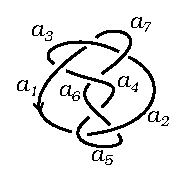
\includegraphics[scale=0.7]{images/7_5}
			\caption{$7_5$}
			\label{fig:7_5}
		\end{minipage}
		\begin{minipage}{0.4\textwidth}
			\centering
	    	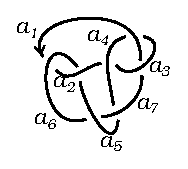
\includegraphics[scale=0.7]{images/7_6}
			\caption{$7_6$}
			\label{fig:7_6}
		\end{minipage}
		\begin{minipage}{0.4\textwidth}
			\centering
	    	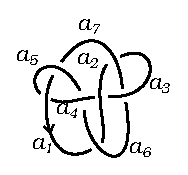
\includegraphics[scale=0.7]{images/7_7}
			\caption{$7_7$}
			\label{fig:7_7}
		\end{minipage}
	\end{figure}

	Presentemos el quandle fundamental de la imagen especular del nudo $3_1$, que vemos en 
	la figura~\ref{fig:3_1m}. El diagrama tiene tres cruces negativos y el
	quandle fundamental es
	\begin{align*}
		Q(m(3_1))=\langle a_1,a_2,a_3:
		a_3\triangleright a_2=a_1,\;
		a_2\triangleright a_1=a_3,\;
		a_1\triangleright a_3=a_2\rangle.
	\end{align*}

	\begin{figure}[ht]
	    \centering
	    \includegraphics[scale=0.7]{images/3_1m}
		\caption{$m(3_1)$.}
    	\label{fig:3_1m}
	\end{figure}

    La figura~\ref{fig:granny} muestra el nudo de la abuela y la
    figura~\ref{fig:square} el nudo cuadrado.  Un cálculo sencillo muestra que 
    el quandle fundamental del nudo de la abuela es
    \begin{multline*}
		Q(3_1\#3_1)=\langle a_1,\dots,a_6:
        a_1\triangleright a_5=a_6,\;
        a_6\triangleright a_1=a_2,\;
        a_2\triangleright a_3=a_4,\\
		a_4\triangleright a_2=a_3,\;
        a_3\triangleright a_4=a_5,\;
        a_5\triangleright a_6=a_1\rangle,
	\end{multline*}
    donde todas las ecuaciones corresponden a cruces positivos, 
    y que el quandle fundamental del nudo cuadrado es
    \begin{multline}
		Q(3_1\#m(3_1))=\langle a_1,\dots,a_6:
        a_5\triangleright a_6=a_1,\;
		a_1\triangleright a_5=a_6,\\
        a_6\triangleright a_1=a_2,\;
        a_4\triangleright a_3=a_2,\;
		a_3\triangleright a_5=a_4,\;
        a_5\triangleright a_4=a_3\rangle,
    \end{multline}
    donde las tres primeras ecuaciones corresponden a los cruces positivos y
   	las tres últimas a los cruces negativos.

%  	\begin{figure}[ht]
% % %		\begin{minipage}{0.3\textwidth}
% % 			\centering
% % 			\includegraphics[scale=0.6]{images/granny}
% % 			\caption{$3_1\#3_1$}
% % 			\label{fig:granny}
% % %		\end{minipage}
% %		\begin{minipage}{0.3\textwidth}
% 			\centering
% 			\includegraphics[scale=0.6]{images/square}
% 			\caption{$3_1\#m(3_1)$}
% 			\label{fig:square}
% %		\end{minipage}
% 	\end{figure}
	\begin{figure}[ht]
		\centering
        \begin{minipage}{0.4\textwidth}
            \centering
			\includegraphics[scale=0.6]{images/granny}
			\caption{$3_1\#3_1$}
			\label{fig:granny}
		\end{minipage}
		\begin{minipage}{0.4\textwidth}
			\centering
			\includegraphics[scale=0.6]{images/square}
			\caption{$3_1\#m(3_1)$}
			\label{fig:square}
		\end{minipage}
    \end{figure}


 
\section{Coloraciones generalizadas}
\label{section:coloreos_generalizados}

    \label{block:counting_invariant}
    Si etiquetamos los arcos de un nudo con los elementos de un quandle $X$ de
    forma tal que en cada cruce se cumplan las relaciones que mencionamos
    en la sección~\ref{block:fundamental_quandle}, o equivalentemente, en la
    figura~\ref{fig:quandle_crossing}, la cantidad de formas en que pueden
    ponerse esas etiquetas quedará invariante después de aplicar movimientos de
    Reidemeister. Esto nos permite ``colorear'' nudos de forma abstracta, donde
    ahora los ``colores'' son en realidad los elementos del quandle $X$. 

    \begin{figure}[h]
		\centering
	    \includegraphics[scale=0.6]{images/quandlecrossing}
		\caption{La regla para colorear con un quandle. Nótese que $a_i\triangleright a_j=a_k$ si y sólo si $a_i\triangleright^{-1}a_k=a_j$.}
        \label{fig:quandle_crossing}
    \end{figure}

	\begin{definition}
		Una \textbf{coloración} del nudo $K$ con el quandle $X$ es un morfismo
		de quandles $Q(K)\to X$. 
	\end{definition}

	Por lo dicho anteriormente, la cantidad de
    morfismos $Q(K)\to X$ es un invariante de nudos.  Este invariante se denota
    por $\mathrm{Col}_X(K)$.  Observemos que siempre existirán al menos $|X|$
    coloraciones del nudo $K$ con el quandle $X$ (las coloraciones triviales).

\begin{example}
    El número de coloraciones con tres colores se puede interpretar como 
    el invariante asociado al
    quandle $\D_3$. Podemos ver la coloración de Fox con $p$ colores 
    como la coloración asociada al quandle $\D_p$. 
\end{example}

\begin{example}
    \label{exa:T}
    Veamos que el nudo $4_1$ puede colorearse de forma no trivial con un
    quandle de Alexander.  Consideremos el cuerpo
    \[
        \F_4=\F_2[\alpha]/(\alpha^2+\alpha+1)=\{0,1,\alpha,\alpha+1\},
    \]
    y sea $X$ el quandle de Alexander de tipo $(4,\alpha)$. Vimos en el
    ejemplo~\ref{exa:4_1:colorings} que las coloraciones con $X$ del diagrama de la
    figura~\ref{fig:4_1} son las soluciones $(a,b,c,d)\in\F_4$ del sistema de
    ecuaciones 
    \begin{equation}
        \label{eq:alexander:4_1}
        \begin{aligned}
            & (1-\alpha)a+\alpha c=d, && (1-\alpha)b+\alpha a=d,\\
            & (1-\alpha)c+\alpha a=b, && (1-\alpha)d+\alpha c=b.
        \end{aligned}
    \end{equation}

    Como $(a,b,c,d)=(0,1,\alpha,\alpha+1)$ es una solución de
    \eqref{eq:alexander:4_1}, el nudo $4_1$ admite entonces al menos una coloración 
    con $X$ no trivial.  Tenemos así otra demostración de la no trivialidad del
    nudo $4_1$. 
\end{example}

%Las coloraciones con quandles de Alexander se llaman \textbf{coloraciones de
%Alexander}. 

\begin{exercise}
	Pruebe que el quandle de conjugación asociado a la matriz $\begin{pmatrix}0
	& 1\\ 2 & 1\end{pmatrix}$ de $\SL(2,\Z_3)$ es isomorfo al quandle de
	Alexander de tipo $(4,\alpha)$ visto en el ejemplo~\ref{exa:T}.  De alguna
	forma, habíamos utilizamos este quandle en el ejemplo~\ref{exa:4_1}.
\end{exercise}

\begin{example}
	En la sección~\ref{block:5_1:fundamental_quandle} presentamos el quandle
	fundamental $Q(5_1)$.  Sea $X$ el quandle de conjugación asociado a
	$(12345)$ en $\Alt_5$.  Un cálculo sencillo muestra que la función
	$Q(5_1)\to X$ definida por 
	\begin{multline*}
        a_1\mapsto (15432),\quad
        a_2\mapsto (12453),\quad
        a_3\mapsto (14352),\\
        a_4\mapsto (15324),\quad
        a_5\mapsto (14523),
	\end{multline*}
	es un morfismo de quandles. Esta función nos permite ``colorear'' el nudo
	$5_1$ con los $5$-ciclos del grupo alternado $\Alt_5$.
\end{example}

\begin{example}
	\label{exa:6_3}
	En la sección~\ref{block:Q(6_3):fundamental_quandle} mostramos las relaciones que
	definen el quandle fundamental del nudo $6_3$. Estas relaciones nos
	permiten demostrar, por ejemplo, que este nudo puede colorearse de forma no
	trivial con el quandle de Alexander de tipo $(7,2)$. En efecto, si
	traducimos
	\eqref{eq:Q(6_3)} a un sistema de ecuaciones obtenemos:
    \begin{equation}
        \label{eq:6_3:sistema_lineal}
        \begin{aligned}
            -a_1+2a_5=a_4, && -a_5+2a_2=a_1, && -a_2+2a_3=a_4,\\
            -a_6+2a_2=a_3, && -a_3+2a_6=a_1, && -a_4+2a_6=a_5.
        \end{aligned}
    \end{equation}
	Como $(a_1,a_2,a_3,a_4,a_5,a_6)=(1,2,0,5,3,4)$ es una solución de
	\eqref{eq:6_3:sistema_lineal}, el nudo $6_3$ puede colorearse de forma no
	trivial con el quandle de Alexander de tipo $(7,2)$. Observemos que si $X$
	es el quandle de Alexander de tipo $(7,2)$, entonces la función $Q(K)\to X$ dada por 
    \begin{align*}
        a_1\mapsto 1, && 
        a_2\mapsto 2, &&
        a_3\mapsto 0, &&
        a_4\mapsto 5, &&
        a_5\mapsto 3, &&
        a_6\mapsto 6
    \end{align*}
    es un morfismo de quandles.
\end{example}

\begin{exercise}
    \label{exercise:varios_pares}
		Pruebe que el quandle de Alexander de tipo $(4,\alpha)$ definido sobre
		el cuerpo
		$\F_4=\F_2[\alpha]/(\alpha^2+\alpha+1)=\{0,1,\alpha,\alpha+1\}$ permite
		distinguir los siguientes pares de nudos: a) $3_1$ y $6_1$; b) $4_1$ y
$5_1$; c) $6_2$ y $7_2$; d) $6_3$ y $7_3$.
\end{exercise}

\begin{exercise}
    \label{exercise:5_2y7_1}
	Pruebe que con una clase de conjugación del grupo alternado $\Alt_5$ es
	posible distinguir los nudos $5_2$ y $7_1$. 
\end{exercise}

\begin{exercise}
    Utilice los resultados de los ejercicios \ref{exercise:colorings},
    \ref{exercise:varios_pares} y \ref{exercise:5_2y7_1} y demuestre que todos los nudos
    de la figura~\ref{fig:knots} son no triviales y distintos.
\end{exercise}

%\label{block:extensions}
Sea $A$ un grupo abeliano (escrito multiplicativamente), sea $X$ un quandle, y sea 
$f\colon X\times X\to A$ una función. Sobre el conjunto $X\times A$ definimos la
operación
\begin{equation}
	\label{eq:extension}
	(x,a)\triangleright (y,b)=(x\triangleright y, bf(x,y))\quad\text{para todo $(x,a),(y,b)\in X\times A$}.
\end{equation}

Es fácil demostrar que la operación \eqref{eq:extension} define una
estructura de quandle sobre $X\times A$ si y sólo si:
\begin{align}
	\label{eq:2cocycle1}&f(x,x)=1,&&\text{para todo $x\in X$},\\
	\label{eq:2cocycle2}&f(x,z)f(x\triangleright y,x\triangleright z)=f(y,z)f(x,y\triangleright z)&&\text{para todo $x,y,z\in X$}.
\end{align}

\medskip
Como ejemplo, demostremos la distributividad. Sean $x,y,z\in X$ y
$a,b,c\in A$. Un cálculo directo nos muestra que 
\begin{align*}
	(x,a)\triangleright( (y,b)\triangleright (c,z))&=(x,a)\triangleright (y\triangleright z, cf(y,z))\\
	&=(x\triangleright(y\triangleright z), cf(y,z)f(x,y\triangleright z)),
\end{align*}
y, por otro lado, 
\begin{align*}
	\left( (x,a)\triangleright(y,b) \right)&\triangleright \left( (x,a)\triangleright (c,z) \right)\\
	&=(x\triangleright y,bf(x,y))\triangleright (x\triangleright z, cf(x,z))\\
&=\left( (x\triangleright y)\triangleright (x\triangleright z) \right), cf(x,z)f(x\triangleright y,x\triangleright z)).
	\end{align*}
	Como $X$ es un quandle, tenemos entonces que la
	condición~\eqref{eq:2cocycle2} es equivalente a la distributividad de la
	operación binaria en $X\times A$.

	\begin{definition}
		\index{$2$-cociclo}
		Una función $f:X\times X\to A$ que satisface las condiciones
		\eqref{eq:2cocycle1} y \eqref{eq:2cocycle2} se llama \textbf{$2$-cociclo
		del quandle $X$} con coeficientes en $A$.  
	\end{definition}

	\begin{definition} 
		El quandle sobre $X\times A$ obtenido con la operación~\eqref{eq:extension} se 
		llama \textbf{extensión abeliana} de $X$ por el grupo abeliano $A$ y el
		$2$-cociclo $f$, y se denota por $X\times_{f}A$.  
	\end{definition}

\begin{example}
    \label{exa:T:2cocycle}
    Supongamos que
    \[
        \F_4=\F_2[\alpha]/(\alpha^2+\alpha+1)=\{0,1,\alpha,\alpha+1\}
    \]
    y sea $X$
    el quandle de Alexander de tipo $(4,\alpha)$.  Sea
    $A=\langle\sigma\rangle=\{1,\sigma\}$ el grupo cíclico de orden dos. La
    función $f\colon X\times X\to A$ dada por 
    \[
    f(x,y)=\begin{cases}
        1 & \text{si $x=y$ o $x=1$ o $y=1$,}\\
        \sigma & \text{en otro caso.}
    \end{cases}
    \]
    es un $2$-cociclo de $X$ con coeficientes en el grupo abeliano $A$. 
\end{example}

\begin{example}
    \label{exa:4cyclesS4}
    Sea $X$ el quandle de conjugación asociado a la clase de $(1234)$ en $\Sym_4$ y sea
    $A=\langle\sigma\rangle=\{1,\sigma,\sigma^2,\sigma^3\}$ el grupo cíclico de
    orden cuatro (escrito multiplicativamente).  La función $f\colon X\times
    X\to A$ dada por la tabla
    \begin{center}
        \begin{tabular}{c|cccccc}
            $f$ & $(1234)$ & $(1432)$ & $(1342)$ & $(1243)$ & $(1324)$ & $(1423)$\tabularnewline
            \hline 
            $(1234)$ & $1$ & $\sigma$ & $\sigma^2$ & $\sigma^2$ &  $\sigma$ & $\sigma^3$\rule{0pt}{3ex}\\ 
            $(1432)$  & $\sigma$ &     1 & $\sigma^2$ &     1 & $\sigma^3$ & $\sigma^3$\\
            $(1342)$ & $\sigma^2$ &  $\sigma$ &     1 &  $\sigma$ & $\sigma^2$ & $\sigma^3$\\
            $(1243)$ & $\sigma^3$ &  $\sigma^2$ &  $\sigma$ &     1 &     $1$ & $\sigma^3$\\
            $(1324)$ & $\sigma$ &  $\sigma$ &  $\sigma$ &  $\sigma$ &     $1$ &  $\sigma$\\
            $(1423)$ & $1$ &     $1$ &     $1$ &     $1$ &  $\sigma$ &     $1$
        \end{tabular}
    \end{center}
    es un $2$-cociclo de $X$ con coeficientes en $A$.
\end{example}

\begin{definition}
	\label{$2$-cociclos!cohómologos}
	\label{$2$-cociclos!equivalentes}
	Un $2$-cociclo $f\colon X\times X\to A$ es un \textbf{coborde} si existe una función 
	$\gamma\colon X\to A$ tal que $f(x,y)=\gamma(x\triangleright
	y)\gamma(y)^{-1}$ para todo $x,y\in X$.
	Dos $2$-cociclos $f$ y $g$ son \textbf{cohomólogos} (o equivalentes) si
	existe $\gamma\colon X\to A$ tal que 
	\[
		f(x,y)=\gamma(x\triangleright y)g(x,y)\gamma(y)^{-1}
	\]
	para todo $x,y\in X$.  
\end{definition}

Cada $2$-cociclo de un quandle $X$
nos permite definir una extensión abeliana de $X$. Estos $2$-cociclos son
en realidad $2$-cociclos en una teoría de cohomología de quandles
\cite{MR1990571}. Tal como pasa en la teoría de grupos, las clases de
equivalencia de extensiones abelianas del quandle $X$ por el grupo abeliano
$A$ están en correspondencia biyectiva con las clases de equivalencia de
$2$-cociclos de $X$ con coeficientes en $A$. La teoría de extensiones
abelianas de quandles tiene además aplicaciones a la teoría de nudos
\cite{MR2008876}.  Para más información sobre la teorías de extensiones y
(co)homologías de quandles referimos a \cite{MR1994219}.

\begin{example}
    \label{exa:granny_vs_square:2}
    \index{Nudo!de la abuela}
    \index{Nudo!cuadrado}
	Recordemos el nudo de la abuela y el nudo cuadrado de la
	figura~\ref{fig:granny_and_square}. En el
	ejercicio~\ref{exercise:granny_and_square} vimos que estos nudos tienen grupos
	fundamentales isomorfos. Sin embargo, como veremos a continuación, estos
	nudos no son equivalentes.  Sean $X$ el quandle de conjugación asociado a
	la clase de $(1234)$ en $\Sym_4$ y $f$ el $2$-cociclo de $X$ que vimos en el
	ejemplo~\ref{exa:4cyclesS4}.  Consideremos la extensión $X\times_fA$ dada
	por
    \[
        (x,\sigma^i)\triangleright (y,\sigma^j)=(x\triangleright y,\sigma^jf(x,y))
        \quad\text{para todo $x,y\in X,\;i,j\in\{0,\dots3\}$.}
    \]

    La extensión abeliana
    $X\times_fA$ nos permite distinguir el nudo de la abuela del nudo cuadrado.  Un
    cálculo nos muestra que para el nudo de la abuela se tiene
	\begin{equation}
		\label{eq:24}
    	\mathrm{Col}_{X\times_fA}(3_1\#3_1)=24,
	\end{equation}
    y que para el nudo cuadrado, en cambio, se tiene 
	\begin{equation}
		\label{eq:408}
    	\mathrm{Col}_{X\times_fA}(3_1\#m(3_1))=408.
	\end{equation}
	Vimos en el ejercicio~\ref{exercise:granny_and_square} que el nudo de la abuela
	es trivial si y sólo si el nudo cuadrado lo es. Esta observación y las
	fórmulas~\eqref{eq:24} y~\eqref{eq:408} implican que estos nudos son no
	triviales y distintos.
\end{example}

\section{Invariantes por $2$-cociclos}
\label{section:cocycles}

A fines del siglo XX, S. Carter, D. Jelsovsky, S. Kamada, L. Langford y M.
Saito anunciaron la construcción de un nuevo invariante de nudos: el invariante
por $2$-cociclos.

Fijemos un grupo abeliano $A$ (escrito multiplicativamente) y un nudo $K$.
Sean $X$ un quandle finito, $\mathcal{C}\colon Q(K)\to X$ una coloración de $K$ y 
$f\colon X\times X\to A$ 
un $2$-cociclo de $X$ con coeficientes en $A$. En cada cruce como el que vemos en la
figura~\ref{fig:crossings} se define el \textbf{peso de Boltzmann}
$\omega_f(\mathcal{C},\chi)$ (con respecto a la coloración $\mathcal{C}$, al
$2$-cociclo $f$ y al cruce $\chi$) como el elemento de $A$ dado por la
expresión 
\[
	\omega_f(\mathcal{C},\chi) =f(a_i,a_j)^{\mathrm{signo}(\chi)}.
\]

\begin{definition}
	\index{Función de partición}
	\index{Invariantes!dados por quandles y $2$-cociclos}
	La \textbf{función de partición} $\Phi_{X,f}(K)$ del nudo $K$ (asociada al
	quandle $X$ y al $2$-cociclo $f$) es la expresión
	\begin{equation}
		\label{eq:cocycle_invariant}
		\Phi_{X,f}(K)=\sum_{\mathcal{C}}\prod_{\chi}\omega_f(\mathcal{C},\chi),
	\end{equation}
	donde el producto se toma sobre todos los cruces $\chi$ que tiene el
	diagrama del nudo $K$ y la suma se toma sobre todos las coloraciones
	$\mathcal{C}$ de $K$ dadas por el quandle $X$.  
\end{definition}

La fórmula~\eqref{eq:cocycle_invariant} define un elemento de $\Z[A]$, el
anillo de grupo de $A$.

\begin{theorem}
    La función de partición $\Phi_{X,f}$ es un invariante de nudos. 

    \begin{proof}
        Tenemos que demostrar que el producto de los pesos de Boltzmann es
        invariante bajo las versiones orientadas de los movimientos de
        Reidemeister. 

        Consideremos el primer movimiento de Reidemeister. Tal como muestra la
        figura~\ref{fig:oriented_R1}, hay dos orientaciones posibles para tener
        en cuenta.  En ambos casos, si suponemos que estas cuerdas llevan la
        etiqueta $a\in X$, entonces en el único cruce $\chi$ que tiene el
        diagrama tendremos el valor $f(a,a)^{\text{signo}(\chi)}$. Como $f$ es
        un $2$-cociclo, $f(a,a)=1$. Luego, el primer movimiento de Reidemeister
        deja invariante al producto de los pesos de Boltzmann.
    
        Consideremos ahora el segundo movimiento. Aquí tenemos cuatro posibles
        diagramas orientados, similares a los que se ve en la
        figura~\ref{fig:oriented_R2}.  Si etiquetamos la cuerda que pasa por
        arriba con $a\in X$ y la cuerda entrante que pasa por debajo con $b\in
        X$ entonces, como para ambos diagramas tenemos un cruce positivo y uno
        negativo, el producto de los pesos de Boltzmann es
        $f(a,b)f(a,b)^{-1}=1$. Luego, el segundo movimiento de Reidemeister
        también deja invariante al producto de los pesos de Boltzmann.

        Para finalizar, tenemos que demostrar que el tercer movimiento de
        Reidemeister deja invariante al producto de los pesos de Boltzmann.
        Como vimos en la sección~\ref{block:quandle_proof}, hay ocho casos para verificar.
        Hagamos como ejemplo el caso que se corresponde con la
        figura~\ref{fig:oriented_R3b} y dejemos el resto como ejercicio.
        \begin{figure}[h]
			\centering
		    \includegraphics[scale=0.6]{images/oriented_R3b}
            \caption{Otra de las configuraciones posibles para el tercer
            movimiento de Reidemeister.}
            \label{fig:oriented_R3b}
        \end{figure}

	    Si calculamos el producto de los pesos de
        Boltzmann sobre los tres cruces que tienen los diagramas de la
        figura~\ref{fig:oriented_R3b} vemos que este producto es invariante por
        el tercer movimiento de Reidemeister si y sólo si
        \[
        f(a,b\triangleright c)f(b,c)f(a,b)=f(a,b)f(a\triangleright b,a\triangleright c)f(a,c).
        \]
        Como $A$ es un grupo abeliano, al cancelar $f(a,b)$ en ambos miembros 
        obtenemos el resultado deseado.
    \end{proof}
\end{theorem}

\label{block:cocycles_and_colorings}
Los invariantes por quandles y $2$-cociclos son una extensión de los invariantes dados por
coloraciones con quandles: si $f$ es un coborde (y por tanto cohomólogo al 2-cociclo constante igual a uno) 
entonces
$\Phi_{X,f}(K)=\Phi_{X,1}(K)=\mathrm{Col}_X(K)$ para todo nudo $K$.	Esta afirmación puede
generalizarse: si $f$ y $g$ son cohomólogos entonces $\Phi_{X,f}=\Phi_{X,g}$.
Para las demostración referimos a la proposición 4.5 de~\cite{MR1990571}.

\begin{example}
	\label{exa:2cocycle:prime_knots}
    Sean $X$ el quandle de Alexander de tipo $(4,\alpha)$ y $f$ el $2$-cociclo
    que vimos en el ejemplo~\ref{exa:T:2cocycle}.  Calculamos  
    $\Phi_{X,f}$ para los nudos de la figura~\ref{fig:knots}:
    \[
    \Phi_{X,f}(K)=\begin{cases}
        4+12\sigma & \text{si $K\in\{3_1,4_1,7_2,7_3\}$},\\
        4 & \text{en otro caso}.
    \end{cases}
    \]
\end{example}

\begin{example}
	\label{exa:2cocycle:3_1andm(3_1)}
    En este ejemplo vamos a distinguir el nudo $3_1$ de su imagen especular
    $m(3_1)$, ver figura~\ref{fig:trefoil_and_mirror}.  Consideremos el quandle
    $X$ y el $2$-cociclo $f$ de $X$ que vimos en el
    ejemplo~\ref{exa:4cyclesS4}.  Un cálculo directo muestra que
    \[
    \Phi_{X,f}(3_1)=6+24\sigma^3,\quad
    \Phi_{X,f}(m(3_1))=6+24\sigma.
    \]
    Esto nos dice que los nudos $3_1$ y $m(3_1)$ no son equivalentes. 
\end{example}

\begin{example}
	\label{exa:granny_vs_square:3}
    \index{Nudo!de la abuela}
    \index{Nudo!cuadrado}
	Vamos a dar otra prueba de que el nudo de la abuela no es equivalente al nudo cuadrado. 
    Como hicimos en el ejemplo anterior, vamos a utilizar el quandle $X$ y 
    el $2$-cociclo $f$ de $X$ que vimos en el ejemplo~\ref{exa:4cyclesS4}.  El
    invariante dado por $X$ y el $2$-cociclo $f$ para el nudo de la abuela es
    \[
    \Phi_{X,f}(3_1\#3_1)=6+48\sigma+96\sigma^2,
    \]
    mientras que para el nudo cuadrado es 
    \[
    \Phi_{X,f}(3_1\#m(3_1))=102+24\sigma+24\sigma^3.
    \]
    Esto nos muestra que el nudo de la abuela no es equivalente al nudo
    cuadrado.
\end{example}

\bibliographystyle{abbrv}
\bibliography{refs}

%\printindex
\end{document}


